%\documentclass[danish,12pt,a4paper]{report}
\documentclass[danish,12pt,a4paper,twoside, openright]{report}

\usepackage[utf8]{inputenc}					
\usepackage[danish]{babel}	% Dokumentets sprog
\usepackage[T1]{fontenc}		
\usepackage{amsmath,amsthm,amssymb,amsfonts,bm}
\usepackage{ragged2e,anyfontsize}
\usepackage{etex}
\usepackage[titletoc]{appendix}
\usepackage{thmtools}
\usepackage[makeroom]{cancel}
\usepackage{placeins}
\usepackage{multirow}
\usepackage{mathtools}
\usepackage[danish]{varioref}
\usepackage[numbers]{natbib}
\usepackage{dirtytalk}
\usepackage{blindtext}
\RequirePackage{etex}
\usepackage{graphicx}
\usepackage{flafter}
\usepackage{float}
\usepackage{makecell}
\usepackage{lastpage}
\usepackage{fancyhdr}
\usepackage{etoolbox}
\usepackage{mdframed}
\usepackage{multicol}
\usepackage{enumitem}
\usepackage[a4paper]{geometry}
\usepackage{a4wide}
\usepackage{parskip}
\usepackage{booktabs}
\usepackage{rotating}
\usepackage{colortbl}
\usepackage{textcomp}
\usepackage{tabularx}
\usepackage{url}
\usepackage{hyperref}
\usepackage{tasks}
\usepackage{commath}
\usepackage{calc}
\usepackage{indentfirst}
\usepackage[hypcap=false]{caption}
\usepackage[official]{eurosym}
\usepackage{listings}
\renewcommand{\lstlistingname}{Korollar}
\RequirePackage{silence}
\WarningFilter{remreset}{The remreset package}


%matricer 
\usepackage{blkarray}

%Fikser underfull og overfull
\hbadness=10001
\vbadness=10001

%Bibliografi og litteratur
\bibliographystyle{Formalia/vancouver}
\setcitestyle{square}
\usepackage[nottoc,numbib]{tocbibind}

%HERFRA------------
%Symbolregister
\usepackage[intoc, danish]{nomencl}
\makenomenclature
\renewcommand{\nomname}{Symbolregister}
\setlength{\columnsep}{1cm}
\setlength{\nomitemsep}{-1pt}

\makeatletter
\newif\if@nomlist

\newcommand*\nomlist{%
  \@nomlisttrue
  \list{}{%
    \labelwidth\nom@tempdim
    \leftmargin\labelwidth
    \advance\leftmargin\labelsep
    \itemsep\nomitemsep
    \let\makelabel\nomlabel}}

\renewcommand*\thenomenclature{%
  \@ifundefined{chapter}%
    {\section*{\nomname}\if@intoc\addcontentsline{toc}{section}{\nomname}\fi}%
    {\chapter*{\nomname}\if@intoc\addcontentsline{toc}{chapter}{\nomname}\fi}%
  \nompreamble
  \@nomlistfalse
}
\renewcommand\nomgroup[1]{%
  \if@nomlist\endlist\end{multicols}\fi
  \ifx#1A\relax
    \def\nomgroupname{Indledning}%
    \else
    \ifx#1B\relax
    \def\nomgroupname{Sandsynlighed}%
    \else
    \ifx#1C\relax
      \def\nomgroupname{Markov-kæder}%
    \else
    \ifx#1D\relax
      \def\nomgroupname{Beregning af $\bm{e^{tA}}$}%
    \else
    \ifx#1E\relax
      \def\nomgroupname{Stabilitet}%
    \else
    \ifx#1F\relax
      \def\nomgroupname{Problemløsning}% 
      % Her kan man indsætte flere afsnit ved at fortsætte if-else statementet, husk at slutte med \fi for at slutte end-if-else
    \else 
       \def\nomgroupname{Diverse}%
      \fi
      \fi
      \fi
      \fi
    \fi
  \fi
  \begin{multicols}{2}[\raggedcolumns\noindent\large\textbf{\textsf{\nomgroupname}}]
  \nomlist
}
\renewcommand*\nompreamble{}
\renewcommand*\nompostamble{\end{multicols}}
\makeatother
%HERTIL------------------------ danke

%Gør indholdsfortegnelse og bibliografi dansk
\addto\captionsdanish{
	\renewcommand\contentsname{Indholdsfortegnelse}	
	\renewcommand{\bibname}{Bibliografi}
}
%Subsubsections i indholdsfortegnelse (ikke nummereret)


%%%% ORDDELING %%%%
\hyphenation{In-te-res-se e-le-ment}

%Sidehoved
\setlength{\headheight}{15pt}
\pagestyle{fancy}
\fancyhf{}
\renewcommand{\chaptermark}[1]{ \markboth{\thechapter.\ #1}{}}
\fancyheadoffset{0pt}
\lhead{\nouppercase \leftmark}
\rhead{Aalborg Universitet}
\renewcommand{\chaptermark}[1]
        {\markboth{#1}{}}
\renewcommand{\sectionmark}[1]
        {\markright{\thesection\ #1}}
\lfoot[\fancyplain{}{\bfseries\thepage}]
    {\fancyplain{}{}}
\rfoot[\fancyplain{}{}]%
    {\fancyplain{}{\bfseries\thepage}}
\patchcmd{\chapter}{plain}{fancy}{}{}

%Kapiteludseende
\usepackage{xcolor}
\usepackage{titlesec, blindtext, color}
\definecolor{gray75}{gray}{0.75}
\newcommand{\hsp}{\hspace{20pt}}
\titleformat{\chapter}[hang]{\huge\bfseries}{\thechapter\hsp\textcolor{gray75}{|}\hsp}{0pt}{\huge\bfseries}
\titlespacing*{\chapter}{0pt}{5pt}{25pt}

% Define a simple command to use at the start of a table row to make it have a shaded background
\newcommand{\gray}{\rowcolor[gray]{.9}}

\usepackage{textcomp}
\usepackage{url}
\usepackage{hyperref}

%TikZ
\usepackage{tikz}
\usetikzlibrary{automata, positioning}
\usetikzlibrary{matrix}
\usetikzlibrary{decorations.markings}
\usepackage{stackengine}
\usetikzlibrary{arrows, petri, topaths,graphs,graphs.standard,arrows.meta}
\tikzstyle{arrow} = [thick,->,>=stealth]
\usepackage{tkz-berge}
\usepackage[position=top]{subfig}
\usepackage{verbatim}
\usepackage{pgfplots}
\pgfplotsset{compat=1.15}
\tikzset{->-/.style={decoration={
  markings,
  mark=at position #1 with {\arrow{>}}},postaction={decorate}}} % Midtvejspil
\usepackage{pgfplots, pgfplotstable}



%---- pseudocode 
\usepackage{algorithm}
\usepackage[noend]{algpseudocode}

\usepackage{framed}
\definecolor{myGray}{HTML}{F9F9F9}
\renewenvironment{leftbar}[4][\hsize]
{\def\FrameCommand
    {{\color{#2}\vrule width #4pt}
        \hspace{-8pt}
        \fboxsep=\FrameSep\colorbox{#3}}
    \MakeFramed{\hsize#1\advance\hsize-\width\FrameRestore}}
{\endMakeFramed}

\algnewcommand\algorithmicforeach{\textbf{for each}}
\algdef{S}[FOR]{ForEach}[1]{\algorithmicforeach\ #1\ \algorithmicdo}

%Sætninger, definitioner, mm. general stil
\declaretheoremstyle[
    % spaceabove=14pt, 
    % spacebelow=6pt, 
    headfont=\normalfont\bfseries, 
    bodyfont = \normalfont,
    postheadspace=2mm, 
    headpunct={.}]{mystyle}
    
%Sætning    
\declaretheorem[name={Sætning}, style=mystyle,numberwithin=section]{thm}
\newenvironment{thmx}[1]
    {\begin{leftbar}{black}{myGray}{3}\begin{thm}#1}{\end{thm}\end{leftbar}}
%Definition
\declaretheorem[name={Definition}, style=mystyle,sibling=thm]{defni}
\newenvironment{defn}[1]
    {\begin{leftbar}{black}{myGray}{3}\begin{defni}#1}{\end{defni}\end{leftbar}}
%Eksempel
\declaretheorem[name={Eksempel}, style=mystyle,sibling=thm]{exmp}
\newenvironment{eks}[1]
    {\begin{leftbar}{gray}{white}{3}\begin{exmp}#1}{\end{exmp}\end{leftbar}}
%Lemma
\declaretheorem[name={Lemma}, style=mystyle,sibling=thm]{lema}
\newenvironment{lem}[1]
    {\begin{leftbar}{black}{myGray}{3}\begin{lema}#1}{\end{lema}\end{leftbar}}
%Proposition
\declaretheorem[name={Proposition}, style=mystyle,sibling=thm]{prop}
\newenvironment{pro}[1]
    {\begin{leftbar}{black}{myGray}{3}\begin{prop}#1}{\end{prop}\end{leftbar}}
%Korollar
\declaretheorem[name={Korollar}, style=mystyle,sibling=thm]{koro}
\newenvironment{kor}[1]
    {\begin{leftbar}{black}{myGray}{3}\begin{koro}#1}{\end{koro}\end{leftbar}}

%Bevis
\declaretheoremstyle[
    spaceabove=14pt, 
    spacebelow=6pt, 
    headfont=\normalfont\bfseries, 
    bodyfont = \normalfont,
    postheadspace=1mm, 
    qed=$\blacksquare$, 
    headpunct={.}]{bevisstyle}
\declaretheorem[name={Bevis}, style=bevisstyle,numbered=no]{bev}

%Inline graphics
\newlength\myheight
\newlength\mydepth
\settototalheight\myheight{Xygp}
\settodepth\mydepth{Xygp}
\setlength\fboxsep{0pt}
\newcommand*\inlinegraphics[1]{%
  \settototalheight\myheight{Xygp}%
  \settodepth\mydepth{Xygp}%
  \raisebox{-\mydepth}{\includegraphics[height=\myheight]{#1}}}


%Kommandoer, som gør jeres liv nemmere, når I skriver. Pas på med at lave for mange kommandoer selv
%da det kan være træls for jer når I skal indsende MWE (minimal working examples) ind i fx stackexchange
\usepackage{bbm}
\newcommand{\R}{\mathbb{R}}
\newcommand{\1}{\mathbbm{1}}
\newcommand{\Z}{\mathbb{Z}}
\newcommand{\N}{\mathbb{N}}
\newcommand{\C}{\mathbb{C}}
\renewcommand{\d}{\mathrm{d}}
\newcommand{\eps}{\varepsilon}
\newcommand{\e}{\mathrm{e}}
\newcommand{\E}{\mathcal{E}}
\newcommand{\tr}{\mathrm{tr }}
\newcommand{\F}{\mathcal{F}}
\renewcommand{\L}{\mathcal{L}}
\newcommand{\m}{\cdot}

\newcommand{\I}{I} % :))

\def\partautorefname{Del}
\def\chapterautorefname{Kapitel}
\def\sectionautorefname{Afsnit}
\def\subsectionautorefname{Underafsnit}
\def\figureautorefname{Figur}
\def\tableautorefname{Tabel}
\def\algorithmautorefname{Algoritme}
\def\lstinputlistingautorefname{Korollar}
\def\itemautorefname{Sætning}
\def\equationautorefname{Ligning}


\def\env@matrix{\hskip -\arraycolsep
  \let\@ifnextchar\new@ifnextchar
  \array{*\c@MaxMatrixCols c}}
  
\newcolumntype{L}[1]{>{\raggedright\let\newline\\\arraybackslash\hspace{0pt}}m{#1}}
\newcolumntype{C}[1]{>{\centering\let\newline\\\arraybackslash\hspace{0pt}}m{#1}}
\newcolumntype{R}[1]{>{\raggedleft\let\newline\\\arraybackslash\hspace{0pt}}m{#1}}



\newcommand\invisiblesection[1]{%
  \refstepcounter{section}%
  \addcontentsline{toc}{section}{\protect\numberline{\thesection}#1}%
  \sectionmark{#1}}
  
  %---- pseudocode 
 \usepackage{algorithm}
\usepackage[noend]{algpseudocode}
\usepackage{listings}
\usepackage{lineno, blindtext}
\renewcommand{\lstlistingname}{Kildekode}
%\usepackage{algorithm2e}
\renewcommand{\gets}{:=}
%\usepackage{algorithmic}
\usepackage{emptypage}

\raggedbottom

\def\hmath$#1${\texorpdfstring{{\rmfamily\textit{#1}}}{#1}}



\begin{document} 

\hbadness=99999
\vbadness=99999

\newcommand{\clearemptydoublepage}{\newpage{\pagestyle{empty}\cleardoublepage}} 

\pdfbookmark[0]{Front page}{label:frontpage}%
\begin{titlepage}

\thispagestyle{empty}

\newcommand{\HRule}{\rule{\linewidth}{0.5mm}}

\center

\textsc{}\\[2.5cm]
    
\textsc{\textbf{\LARGE Aalborg Universitet}}\\[1.5cm]

\textsc{\textbf{\Large 4. semester}}\\[0.5cm]

\textsc{\textbf{\large Matematik-Økonomi}}\\[0.5cm]

\textsc{\textbf{\large P4-projekt}}\\[0.5cm]

\textsc{\textbf{\large }}\\[0.5cm]

\HRule \\[0.4cm]

{\huge \bfseries Markov Processes and Decision Theory}\\[0.4cm]

\HRule\\[1.5cm]

\textbf{\large 28/05-2021}\\[1cm]


\includegraphics[height=5cm]{Formalia/AAU-logo-stud-DK-RGB.pdf}

\vfill

\end{titlepage}
\pagebreak
\thispagestyle{empty}
\phantom{a}
\clearpage

% Dette er LaTeX-versionen af titelbladet for TNB studenterrapporter
% Filen kræver:
% Universitetets logo:  AAU-logo-stud-UK eller AAU-logo-stud-DK
% Synopsis: En fil ved navn synopsis.tex

% Udarbejdet af: Jesper Nørgaard (jesper@noergaard.eu) 10. april 2012

\phantomsection
\pdfbookmark[0]{Titelblad}{titelblad}
\thispagestyle{empty}

\begin{minipage}[t]{0.48\textwidth}
\vspace*{-25pt}			%\vspace*{-9pt}

\includegraphics[height=4cm]{Formalia/AAU-logo-stud-DK-RGB.pdf}
\end{minipage}
\hfill
\begin{minipage}[t]{0.48\textwidth}
{\small 
\textbf{Institut for Matematiske Fag}\\
Matematik\\
Skjernvej 4A \\
9220 Aalborg Øst \\
\href{http://math.aau.dk}{http://math.aau.dk}}
\end{minipage}

\vspace*{1cm}

\begin{minipage}[t]{0.48\textwidth}
\textbf{Titel:} \\[5pt]\hspace{2ex}
{Markov Processes and Decision Theory}
\bigskip

\textbf{Projekt:} \\[5pt]\hspace{2ex}
P4-projekt
\bigskip

\textbf{Projektperiode:} \\[5pt]\hspace{2ex}
1. februar 2021 - 28 maj 2021
\bigskip

\textbf{Projektgruppe:} \\[5pt]\hspace{2ex}
Gruppe-nummer - f21mmf2
\bigskip

\textbf{Deltagere:} \\[5pt]%\hspace*{2ex}
Jonathan Pedersen\\%\hspace*{2ex}
Julie Tømmerby Thomsen\\%\hspace*{2ex}
Mikkel Irgens Prior Nielsen \\%\hspace*{2ex}
Oliver Christensen\\%\hspace*{2ex}
Sandra Helweg Sørensen\\
%Navn6\\%\hspace*{2ex}

\textbf{Vejleder:} \\[5pt]%\hspace*{2ex}
Toke Zinn \\

\textbf{Sidetal: \pageref{LastPage} + forside} \\ 
\textbf{Afsluttet 27/05-2020}

\end{minipage}
\hfill
\begin{minipage}[t]{0.5\textwidth}
\textbf{Synopsis:} \\[5pt]
This paper examines how to determine the optimal consumption and maximal reward for a consumer in a given period. Furthermore, it studies how the probability of unemployment, interest rate and loan affect the optimal consumption and maximal reward. The Consumer Problem is a Markov Decision Process and therefore, the optimal consumption and maximal reward can be determined using backward induction and the Bellman equation. To arrive at this conclusion and to implement the probability of unemployment, it is necessary to introduce basic concepts within probability theory such as conditional probability, expected value and Markov-chains. Moreover, Markov Decision Processes will be examined and implemented within the Consumption Problem using Python.
From this, an inverse relationship between unemployment and total reward has been found, while the reasonable consumer has a positive relationship between consumption and interest rate. Furthermore, the loan restriction and ratio between the lendingrate and depositrate affect the reward and the consumption.




 % Skriv synopsis i dette dokument
\end{minipage}
\hspace*{2ex}

\vfill

{\footnotesize \textit{Rapportens indhold er frit tilgængeligt, men offentliggørelse (med kildeangivelse) må kun ske efter aftale med forfatterne.}}

\pagebreak
\phantom{a}
\thispagestyle{empty}
\clearemptydoublepage

\setcounter{page}{1}
\pagenumbering{roman}
\section*{Forord}
\addcontentsline{toc}{chapter}{\protect\numberline{}Forord}


Projektperioden er forløbet fra 01/02-2021 - 28/05-2021, og er skrevet at matematik-økonomi studerende på Aalborg Universitet. Det antages, at læseren mindst er 4. semesters studerende på en matematisk uddannelse, og kender dermed begreber som konvergens, ligevægt med mere. \\

\large\textbf{Læservejledning} \normalsize \newline
Referencer er skrevet i begyndelsen af hvert afsnit og henviser til litteraturlisten i slutningen af projektet. Henvisninger er skrevet efter Vancouvermetoden, og skrives derfor: [kildenummer, sidetal].     % Vancover-metoden

\bigskip

\textcolor{white}{tekst}

\begin{minipage}[L]{0.45\textwidth}
 \centering
 \rule{\textwidth}{0.5pt}\\
  Jonathan Pedersen\\
 {\footnotesize jlpe19@student.aau.dk}
\end{minipage}
\hfill
\begin{minipage}[H]{0.45\textwidth}
 \centering
 \rule{\textwidth}{0.5pt}\\
  Julie Tømmerby Thomsen\\
 {\footnotesize jtth19@student.aau.dk}
\end{minipage}
\vspace{3\baselineskip}


\begin{minipage}[L]{0.45\textwidth}
 \centering
 \rule{\textwidth}{0.5pt}\\
 Mikkel Irgens Prior Nielsen\\
 {\footnotesize mipn19@student.aau.dk}
\end{minipage}
\hfill
\begin{minipage}[H]{0.45\textwidth}
 \centering
 \rule{\textwidth}{0.5pt}\\
  Oliver Christensen\\\
 {\footnotesize ochri19@student.aau.dk}
\end{minipage}
\vspace{3\baselineskip}


\begin{minipage}[H]{0.45\textwidth}
 \centering
 \rule{\textwidth}{0.5pt}\\
 Sandra Helweg Sørensen\\
 {\footnotesize shsa19@student.aau.dk}
\end{minipage}



\pagebreak
%Symbolregister

% Symbolregisteret kan opdeles som set nedenfor, ved at indsætte \nomenclature[A]{$mit-symbol$}{forklaring} indsættes det under kategori A, kategori kan laves i preamble under symbolregister, hvis ikke et symbol får en kategori gives den "other".

% Eksempel på et symbolregister:

% A = Indledning/Problemanalyse/Problemformulering


% B = Sandsynlighed
%Mængder
\nomenclature[B,01]{$\Omega$}{Et udfaldsrum}
\nomenclature[B,02]{$\omega$}{Element af udfaldsrummet}
\nomenclature[B,04]{$A, B$}{Hændelser}
\nomenclature[B,03]{$\F$}{Hændelsesrum}
\nomenclature[B,05]{$\emptyset$}{Den tomme mængde}
\nomenclature[B,08]{$\R$}{De reelle tal}
\nomenclature[B,06]{$P(\cdot)$}{Sandsynlighedsmål}
\nomenclature[B,09]{$A_k, B_k$}{Den $k$'te hændelse}
\nomenclature[B,11]{$P(A \mid B)$}{Sandsynligheden for $A$ givet $B$}
\nomenclature[B,10]{$k,n,i,j$}{Tællevariabler}
\nomenclature[B,00]{$\E$}{Tilfældigt eksperiment}
\nomenclature[B,12]{$X, Y$}{Diskrete tilfældige variabler}
\nomenclature[B,13]{Range$(\cdot)$}{Billedet af en diskret tilfældig variabel}
\nomenclature[B,07]{$(\Omega,\F, P)$}{Sandsynlighedsrum}
\nomenclature[B,14]{$X^{-1}$}{Urbilledet af $X$}
\nomenclature[B,15]{$p_X(\cdot)$}{Frekvensfunktionen til $X$}
\nomenclature[B,16]{$\mathcal{Y}$}{En mængde}
\nomenclature[B,16]{$F_X(\cdot)$}{Fordelingsfunktion til $X$}
\nomenclature[B,18]{$g(\cdot)$}{Vilkårlig reel funktion funktion}
\nomenclature[B,17]{$E[\cdot]$}{Den forventede værdi}
\nomenclature[B,19]{$E[X \mid Y]$}{Den forventede værdi for $X$ givet $Y$}
\nomenclature[B,20]{Var$[\cdot]$}{Varians}
\nomenclature[B,21]{$\sigma$}{Standardafvigelsen}

%Diverse


% C = Markov-kæder
\nomenclature[C,01]{$\bm X$}{En sekvens af diskrete tilfældige variabler }
\nomenclature[C,02]{$S$}{Tilstandsrummet}
\nomenclature[C,03]{$T$}{Indeksmængden}
\nomenclature[C,04]{$j, i$}{Tilstande i tilstandsrummet}
\nomenclature[C,05]{$t, m, r$}{Indicer i indeksmængden}
\nomenclature[C,06]{$p_{ij}$}{Overgangssandsynligheden for en Markov-kæde}
\nomenclature[C,07]{$\P$}{Overgangsmatricen for en Markov-kæde}
\nomenclature[C,08]{$P(X_0 = i_0)$}{Begyndelses -\\sandsynligheden}
\nomenclature[C,09]{$p_{ij}^{(t)}$}{$t$'te trins overgangssandsynligheden for en Markov-kæde}
\nomenclature[C,10]{$\P^{(t)}$}{$t$'te trins overgangsmatricen for en Markov-kæde}
\nomenclature[C,11]{$i \to j$}{$j$ er tilgængelig fra $i$}
\nomenclature[C,12]{$i \leftrightarrow j$}{$j$ og $i$ kommunikerer}
\nomenclature[C,13]{$\tau_i$}{Antal trin før Markov-kæden besøger $i$}
\nomenclature[C,14]{$d(i)$}{Største fælles divisor af antallet af trin for at vende tilbage til $i$.}
\nomenclature[C,15]{$\bm \pi$}{Invariant fordeling}
\nomenclature[C,16]{$\pi_i$}{Den $i$'te indgang i den invariante fordeling}
\nomenclature[C,17]{$\bm q$}{En sandsynlighedsfordeling}
\nomenclature[C,18]{$q_i$}{Den $i$'te indgang i en sandsynlighedsfordeling}



% \noncleture[BOGSTAV,VÆGT]{symbol}{symbolforklaring}
% Hvor BOGSTAV betegner afsnittet den skal i og VÆGT betegner hvor den skal hen (01 er først og 0n er sidst)

% D =  Markov beslutningsprocesser
\nomenclature[D,01]{$T$}{Mængden af beslutningstidspunkter}
\nomenclature[D,02]{$t$}{Beslutningstidspunkter}
\nomenclature[D,03]{$S$}{Tilstandsrummet}
\nomenclature[D,04]{$s$}{Tilstande}
\nomenclature[D,05]{$S_t$}{Mængden af tilstande til $t$}
\nomenclature[D,06]{$A$}{Beslutningsrummet}
\nomenclature[D,07]{$a$}{Beslutninger}
\nomenclature[D,08]{$A_s$}{Mængden af mulige beslutninger til $s$}
\nomenclature[D,09]{$A_{s,t}$}{Mængden af mulige beslutninger til $s$ og $t$}
\nomenclature[D,10]{$r_t(s,a)$}{Belønning}
\nomenclature[D,11]{$r_t(s,a,s')$}{Belønning afhængig af tilstanden til $t+1$}
\nomenclature[D,12]{$s'$}{Tilstanden til beslutningstidspunktet $t+1$}
\nomenclature[D,13]{$p_t(\cdot \mid s,a)$}{Overgangssandsynlig - \\hedsfunktionen}
\nomenclature[D,14]{$N$}{Sidste beslutningstidspunkt}
\nomenclature[D,15]{$d_t$}{Beslutningsregel}
\nomenclature[D,16]{$h_t$}{Historik}
\nomenclature[D,17]{$H_t$}{Mængden af historikker}
\nomenclature[D,18]{$q_{d_t}(\cdot)$}{Sandsynlighedsfordelingen for mængden af beslutningsregler}
\nomenclature[D,19]{$D_t^K$}{Mængden af beslutningsregler}
\nomenclature[D,20]{$K$}{Klassen af beslutningsregler}
\nomenclature[D,21]{$\Psi$}{Strategi}
\nomenclature[D,22]{$\Pi$}{Mængden af alle strategier}
\nomenclature[D,23]{$\omega$}{Udfaldsvej}
\nomenclature[D,24]{$Z_t, W$}{Diskret tilfældig variabel}
\nomenclature[D,25]{$P^\Psi$}{Sandsynlighedsmål givet en strategi}
\nomenclature[D,26]{$E^\Psi$}{Den forventede værdi givet en strategi}
\nomenclature[D,27]{$v_N^{\Psi}$}{Den forventede totale belønning givet en strategi}
\nomenclature[D,28]{$\Psi^*$}{Den optimale strategi}
\nomenclature[D,29]{$v_N^{\Psi^*}$}{Den forventede totale belønning givet en optimal strategi}
\nomenclature[D,30]{$\Psi^*_\varepsilon$}{Den $\varepsilon$-optimale strategi}
\nomenclature[D,31]{$v_N^{\Psi^*_\varepsilon}$}{Den forventede totale belønning givet en $\varepsilon$-optimal strategi}
\nomenclature[D,32]{$v_N^{*}$}{Den maksimale forventede totale belønning}
\nomenclature[D,33]{$u_t^{\Psi}$}{Den forventede totale belønning givet en strategi fra beslutningstidspunkt $t$}
\nomenclature[D,34]{$u_t^{*}=u_t$}{Den maksimale forventede totale belønning fra beslutningstidspunkt $t$}
\nomenclature[D,35]{$G$}{En vilkårlig diskret mængde}
\nomenclature[D,36]{$z$}{Element i $G$.}
\nomenclature[D,37]{$a^\circ$}{En beslutning}
\nomenclature[D,38]{$\lambda$}{Diskonteringsfaktor}
\nomenclature[D,39]{$v_{N,\lambda}^{\Psi}$}{Den forventede totale diskonterede belønning givet en strategi}


% E =Investeringsproblemet
\nomenclature[E,01]{$T$}{Mængden af beslutningstidspunkter}
\nomenclature[E,02]{$t$}{Beslutningstidspunkter}
\nomenclature[E,03]{$S$}{En opsparing}
\nomenclature[E,04]{$S_t$}{En opsparing til beslutningstidspunkt $t$}
\nomenclature[E,05]{$a_t$}{En beslutning der angiver et forbrug til beslutningstidspunkt $t$}
\nomenclature[E,06]{$A_t$}{Mængden af beslutninger $a_t$}
\nomenclature[E,07]{$\gamma_i$}{Indlånsrenten}
\nomenclature[E,07]{$\gamma_u$}{Udlånsrenten}
\nomenclature[E,08]{$I$}{Indkomst}
\nomenclature[E,09]{$\bm \xi$}{Stokastisk proces for arbejdsstatus}
\nomenclature[E,10]{$\xi$}{Arbejdsstatus til beslutningstidspunkt $t$}
\nomenclature[E,11]{$\alpha$}{Sandsynligheden for at investoren mister sit arbejde i næste beslutningstidspunkt givet, at han er i arbejde i det nuværende beslutningstidspunkt}
\nomenclature[E,12]{$\beta$}{Sandsynligheden for at investoren er arbejdsløs i næste beslutningstidspunkt givet, at han ikke er i arbejde til nuværende arbejdstidspunkt}
\nomenclature[E,13]{$\Delta$}{En diskretseringfaktor}
\nomenclature[E,14]{$L_t$}{Samlede lån indtil $t$}
\nomenclature[E,15]{$L$}{Lånebegrænsning}



% F = Problemløsning

% P = Diverse


\printnomenclature[2.5cm]

% Ja præcis den her :))))))))))))

\tableofcontents

\clearpage
\clearemptydoublepage
\setcounter{page}{1}
\pagenumbering{arabic}


%Indsæt her jeres dokumenter. Lav mapper under afsnit, som har jeres kapitelnavne, og indsæt herunder disse mapper jeres .tex dokumenter

\chapter{Indledning} 
    % Input indledningens main-fil her:
    \section{Problemanalyse}

Alle mennesker, som køber og forbruger varer, kan klassificeres som forbrugere. Enhver forbruger har en opsparing og en indkomst, som udgør et muligt forbrug. En forbruger har et basisforbrug, hvilket er det nødvendige forbrug, herunder vand, varme og husleje. Derudover har forbrugere et varierende forbrug, som er den del af forbruget, der bruges på eksempelvis tøj og møbler. Det varierende forbrug afhænger af den marginale forbrugstilbøjelighed, som bestemmer hvor meget af den disponible indkomst, der forbruges. Da basisforbruget er et nødvendigt forbrug, vil den marginale forbrugstilbøjelighed ikke påvirke dette.

Ved at købe varer og ydelser får forbrugeren en tilfredshed, som måles i nytte. Forbrugere er interesseret i at få så meget tilfredshed som muligt. Derfor skal man som forbruger beslutte, hvor meget der skal spares op, og hvor meget der skal forbruges til et givet tidspunkt for at maksimere sin nytte. Disse beslutninger afhænger blandt andet af forbrugerens nuværende økonomi samt forventningerne til den fremtidige økonomi. Forbrugerens økonomi kan blandt andet blive påvirket af arbejdsstatus, løn, pandemier og finanskriser. Disse faktorer påvirker det varierende forbrug, da den disponible indkomst og den marginale forbrugstilbøjelighed ændres. 

Forbrugere er forskellige, hvilket resulterer i, at hver forbruger har deres egen strategi  til at opnå mest mulig nytte. Nogle forbrugere får mere nytte af at forbruge så meget som muligt i nuet og er derfor ligeglade med indlånsrenten. Andre forbrugere er indifferente i forhold til, om der forbruges nu fremfor senere. Denne type forbruger maksimerer sin nytte ved at have et højt samlet forbrug. Ved en positiv indlånsrente vil denne forbruger dermed maksimere sin nytte ved at forbruge alt til sidst. Typisk er forbrugere mere påpasselige med deres forbrug. Forbrugere får derfor ofte mest nytte af at fordele forbruget ud, så der kan forbruges i hver måned. De ovenstående forbrugstilbøjeligheder kaldes henholdsvis utålmodig, tålmodig og fornuftig, og vil uddybes senere i projektet. 
\pagebreak
\section{Problemafgrænsing}
Problemet hvor en forbruger skal tage beslutninger over en given tidsperiode for at maksimere sin nytte, kaldes forbrugerproblemet, og kan opstilles som en Markov beslutningsproces.

Denne Markov beslutningsproces er en beslutningsmodel, hvor forbrugeren til hvert beslutningstidspunkt skal vælge, hvor meget der skal forbruges. Beløbet som ikke forbruges spares op og kan dermed forbruges til næste beslutningstidspunkt. Forbrugeren skal til ethvert beslutningstidspunkt vælge det forbrug, som maksimerer nytten over hele tidsperioden. %Dette forbrug kan bestemmes ved at anvende baglæns induktion heriblandt Bellman ligningen. 

I dette projekt vil forbruget ikke blive delt op i basis- og varierende forbrug. Det antages, at forbrugerens løn og forventning til arbejdstatus er fast over tidsperioden. Derfor påvirkes disse faktorer blandt andet ikke af pandemier eller finanskriser, som ofte medfører højere arbejdsløshed og lavere løn. Derudover antages det, at den disponible indkomst er lig lønnen, når forbrugeren er i arbejde og nul i de beslutningstidspunkter, hvor han er arbejdsløs. Den disponible indkomst påvirkes dermed ikke af skatteændringer. Sandsynligheden for at være i arbejde vil blive beskrevet ved en Markov-kæde, hvor forbrugerens arbejdsstatus i næste tidsskridt kun afhænger af hans arbejdsstatus i nuværende tidsskridt.

Dette projekt tager udgangspunkt i den fornuftige forbruger, der opnår størst mulig nytte ved at fordele sit forbrug ligeligt mellem beslutningstidspunkterne. Det antages, at det optimale forbrug til hvert beslutningstidspunkt udelukkende afhænger af sandsynligheden for at blive arbejdsløs, forblive arbejdsløs, opsparing og indlånsrente. Når muligheden for at låne penge tilføjes, afhænger forbruget til hvert beslutningstidspunkt også af dette, samt udlånsrenten.

Det er derfor interessant at undersøge, hvordan forbrugerens nytte og forbrug til hvert beslutningstidspunkt påvirkes, hvis sandsynligheden for at blive arbejdsløs, indlånsrenten og muligheden for at låne varierer. 


%For at kunne beskrive Markov-kæderne for forbrugerens %arbejdsstatus og Markov beslutningsprocessen vil der %introduceres begrebet forventet værdi. Derudover %præsenteres begreber som tilfældige variabler og %sandsynlighedsrum.

%for at kunne beskrive forventet værdi, Markov kæder og %Markovbeslutningsprocesser. 

Ud fra ovenstående problemafgrænsning opstilles følgende problemformulering.





 





\input{Afsnit/Indledning/Afgrænsning}

\section{Problemformulering}

En super god problemformulering - Tekst her Tekst her Tekst her 






\chapter{Sandsynlighed}\label{kapitel:sandsynlighed}
I dette kapitel anvendes \cite[s. 1-111]{olofsson2005probability} og \cite[s. 6-32]{oxford}. 

Sandsynlighedsteori kan anvendes inden for blandt andet matematik og økonomi til at beregne sandsynligheden for forskellige udfald. I dette projekt tages der udgangspunkt i en forbruger, hvis arbejdsstatus er beskrevet ved en Markov-kæde. 
For at kunne definere og analysere Markov-kæder introduceres nogle grundlæggende begreber inden for sandsynlighedsteori. Disse begreber defineres i dette kapitel. 

\section{Introduktion}
To primære fortolkninger af sandsynlighed er, at en sandsynlighed er grænsen for den relative frekvenser eller en vis grad af tro. Ud over disse to fortolkninger er det muligt at formulere en mere matematisk præcis definition af hvad sandsynlighed er.

For at kunne beskrive hvad en sandsynlighed mere matematisk præcis, skal begreber som \textit{tilfældighed}, \textit{udfaldsrummet} og \textit{hændelser} først beskrives.

I en situation hvor der sker noget, der ikke er muligt at forudse det præcise udfald kaldes \textit{tilfældig}. Et eksempel på dette kan være, hvis man kaster med en terning, hvor man ikke er sikker på om man slår $1, 2, \cdot$ eller $6$. Dette kaldes for et \textit{tilfældigt eksperiment}. For et tilfældigt eksperiment kan begreberne udfaldsrum og hændelser defineres som følgende

\begin{minipage}\textwidth
\begin{defn}\textbf{Udfaldsrum} %Ny definition
\newline
Mængden af mulige udfald i et tilfældigt eksperiment kaldes et udfaldsrum og bliver noteret, $S$.
\end{defn}
\end{minipage}

Et udfaldsrum kan være \textit{endeligt}, \textit{tællelig uendeligt} og \textit{ikke-tællelig uendeligt}. Endeligt betyder, at udfaldsrummet består af et endeligt antal udfald, hvor der gælder for de to andre, at udfaldsrummet består at et uendeligt antal udfald. Hvis udfaldene er adskilt i punkter som foreksempel $\{1,2,3, \cdots\}$ er udfaldsrummet tællelig, og hvis det derimod er et kontinuum af punkter er det ikke-tællelig. Et eksempel på dette er udfaldsrummet $[0, \infty)$.

\begin{minipage}\textwidth
\begin{defn}\textbf{Hændelse} %Ny definition
\newline
En delmængde af udfaldsrummet, $A \subseteq S$, kaldes en hændelse.
\end{defn}
\end{minipage}

Hvis der for to hændelser $A$ og $B$ gælder at $A \cap B = \varnothing$ kaldes de for \textbf{\textit{disjunkte}}.

Følgende beskriver et eksemplet for udfaldsrummet og hændelser for det tilfældige eksperiment, hvor der kastes med en terning.

\begin{eks} \textbf{} %Nyt eksempel
\newline
Det tilfældige eksperiment går ud på, at man kaster en terning og observerer nummeret.

For dette tilfældige eksperiment vil udfaldene kunne være tallene fra 1 til 6. Dermed vil udfaldsrummet være
\begin{align*}
    S = \{1, 2, 3, 4, 5, 6\}
\end{align*}

Det er også muligt at have to hændelser, når man kaster en terning, hvor den ene hændelse er at få ulige numre og den anden er at få lige numre. Altså er delmængderne at udfaldsrummet følgende
\begin{align*}
    A = \{1, 3, 5\} \quad B = \{2, 4, 6\}
\end{align*}
I dette tilfælde er $A$ og $B$  \textbf{disjunkte}, da $A \cap B = \varnothing$. Altså er det ikke muligt at både $A$ og $B$ kan hænde på samme tid.
\end{eks}

Det er hermed muligt at lave en matematisk definition af sandsynlighed.

\begin{defn}\textbf{Sandsynlighedsregningens grundsætninger} \label{def:sandsynlighedsregningens_grundsætninger}%Ny definition
\newline
Et sandsynlighedsmål er en funktion $P$, 
der tildeler hver hændelse $A$ et tal $P(A)$, der opfylder at
\begin{enumerate}
    \item[(a)] $0 \leq P(A) \leq 1$
    \item[(b)]$P(S) = 1$ og $P(\emptyset)=0$
    \item[(c)] Hvis $A_1, A_2, \cdots$ er en sekvens af parvise \textbf{disjunkte} hændelser, altså at hvis $i \neq j$, så er $A_i \cap A_j = \varnothing$, så gælder det at
\end{enumerate}
\begin{align*}
    P\left(\bigcap_{k=1}^\infty A_k \right) = \sum_{k=1}^\infty P(A_k)
\end{align*}
\end{defn}

Ud fra det sidste aksiom i \autoref{def:sandsynlighedsregningens_grundsætninger} følger det naturligt, at hvis $A_1, A_2, \cdots , A_n$ er en sekvens af parvise \textbf{disjunkte} hændelser så gælder det at
\begin{align*}
    P\left(\bigcap_{k=1}^n A_k \right) = \sum_{k=1}^n P(A_k)
\end{align*}

\textbf{Tænker at vi skriver de regneregler(inklusiv lim) ind vi bruger hen ad vejen. gider ikke lige skrive dem alle sammen ind og bevise dem hvis vi kun anvender 2,3 stykker. samme med regrad to order/replacement}















\section{Betinget sandsynlighed}
Hvis man har ekstra information om en given hændelse, så vil udfaldsrummet indskrænkes - mere formelt:\\
\begin{minipage}\textwidth
\begin{defn}\textbf{Betinget sandsynlighed} %Ny definition
\newline
Lad $B$ være en hændelse sådan at $P(B)>0$. Den \textit{betingede sandsynlighed} af $A$ givet $B$ er defineret som
\begin{align*}
      \displaystyle P(A|B)=\frac{P(A\cap B)}{P(B)}
\end{align*}
\end{defn}
\end{minipage}

\subsection{Uafhængige hændelser}
Hvis to hændelser, $A$ og $B$, er \textit{uafhængige}, vil en betingelse $B$ ikke påvirke sandsynligheden for $A$. Med andre ord, så er den betingede og ubetingede sandsynlighed den samme. Dette har konsekvensen, at $P(A)=P(A|B)\Leftrightarrow P(A\cap B)=P(A)P(B)$. Faktisk kan dette generaliseres til følgende definition:\\
\begin{minipage}\textwidth
\begin{defn}\textbf{Uafhængighed} %Ny definition
\newline
Hændelserne, $A_1,A_2,\dots$ siges at være uafhængige hvis
\begin{align*}
    P(A_{i_1}\cap A_{i_2}\cap\cdots\cap A_{i_k})=P(A_{i_1})P(A_{i_2})\cdots P(A_{i_k})
\end{align*}
for alle følger af heltal, $i_1<i_2<\cdots<i_k, k=2,3,\dots$.
Hvis de ikke er uafhængige er \textit{afhængige}.
\end{defn}
\end{minipage}
\subsection{Total sandsynlighed}
I tilfælde af, at sandsynligheden for en given hændelse er svær at bestemme direkte kan det i nogle tilfælde være hensigtsmæssigt at opdele problemet i termer af betinget sandsynlighed.



\begin{minipage}\textwidth
\begin{thmx} \textbf{Loven om Total Sandsynlighed} \label{sæt:loven_om_total_sandsynlighed} %Ny sætning
\newline
Lad $B_1,B_2,\dots$ være en følge af hændelser, sådan at
\begin{enumerate}[label=(\textbf{\alph*})]
\item $P(B_k)>0$ for $k=1,2,\dots$
\item $B_i$ og $B_j$ er disjunkte når $i\neq j$
\item $S=\bigcup_{k=1}^\infty B_k$
\end{enumerate}
Så for enhver hændelse, $A$ gælder der, at
\begin{align*}
    P(A)=\sum_{k=1}^\infty P(A|B_k)P(B_k)
\end{align*}
\end{thmx}
\end{minipage}
\begin{bev} \textbf{} %Nyt bevis
\newline
Bemærk, at
\begin{align*}
    A=A\cap S=\bigcup_{k=1}^\infty(A\cap B_k)
\end{align*}
i henhold til den distributive lov for uendelige foreningsmængder (se Bilag \ref{Distributive love}). 
Eftersom $A\cap B_1,A\cap B_2,\dots$ er parvis disjunkte fås
\begin{align*}
    P(A)=\sum_{k=1}^\infty P(A\cap B_k)=\sum_{k=1}^\infty P(A|B_k)P(B_k)
\end{align*}
\end{bev}
%By virtue of Proposition 1.2, we realize that the law of total probability is also true for a finite union of events
%Hvis mængden af hændelser er endelig og givet ved $n$, kan man konstruere en uendelig følge af hændelser, sådan at P(\bigcup_{k=n}^\infty B_k)=0.
For $n=2$ gælder der, at hvis $B_1=B$, så følger det at $B_2=B^c$ og følgende korollar fås.
\begin{minipage}\textwidth
\begin{kor} \textbf{} %Nyt korollar
\newline
Hvis $0<P(B)<1$, så er
\begin{align*}
    P(A)=P(A|B)P(B)+P(A|B^c)P(B^c)
\end{align*}
\end{kor}
\end{minipage}
\iffalse
Idét foreningsmængder er kommutative, gælder der, at
$$P(B_j|A)P(A)=P(A|B_j)P(B_j)$$
som må betyde, at
$$P(B_j|A)=\frac{P(A|B_j)P(B_j)}{P(A)}$$

Dette leder op til følgende proposition:\\
\begin{minipage}\textwidth
\begin{pro} \textbf{(Bayes' Formel).} %Ny proposition
\newline
Med samme antagelser som i Loven om Total Sandsynlighed og hvis $P(A)>0$, så gælder der for enhver hændelse, $B_j$, at
\begin{align*}
    P(B_j|A)=\frac{P(A|B_j)P(B_j)}{\sum_{k=1}^\infty P(A|B_k)P(B_k)}
\end{align*}
\end{pro}
\end{minipage}
\begin{bev}
Beviset følger af foregående udregninger.
\end{bev}

Analogt, følger denne korrollar:\\
\begin{minipage}\textwidth
\begin{kor} \textbf{} %Nyt korollar
\newline
Hvis $0<P(B)<1$ og $P(A)>0$, så er
\begin{align*}
    P(B|A)=\frac{P(A|B)P(B)}{P(A|B)P(B)+P(A|B^c)P(B^c)}
\end{align*}
\end{kor}
\end{minipage}
\fi

\section{Tilfældige variabler}

% $S = \{1,2,3\}$
% $\Sigma = \{\emptyset, \{ 1\}, \{ 2\}, \{ 3\},  \{ 1, 2\}, \{ 2,3 \}, \{ 1,3\}, S\}$
% \pagebreak
% Tilfældig variabel:\\
% En tilfældig variabel på $(S,\Sigma, P)$ er en funktion $X:S\to \R$ således at:\\
% $\forall x\in \R : \{s \in S: X(s)\leq x\} \in \Sigma$

% Tilfældig diskret variabel:\\
% Billedet er en tællelig delmængde af $\R$\\
% $\forall x\in \R : \{s \in S: X(s) = x\} \in \Sigma$




% \begin{minipage}\textwidth
% \begin{defn}\textbf{Tilfældig variabel} %Ny definition
% \newline
% En tilfældig variabel er en variabel, $x\in \R$, der får sin værdi fra et tilfældigt eksperiment.
% \end{defn}
% \end{minipage}

% \begin{minipage}\textwidth
% \begin{defn}\textbf{Tilfældig variabel} %Ny definition
% \newline
% Lad $\E$ være et eksperiment med sandsynlighedsrummet $(S, \Sigma, P)$.

% Så er en tilfældig variabel en funktion på sandsynlighedsrummet $X:S\to \R$.


% \end{defn}
% \end{minipage}


En \textit{tilfældig variabel}, $X$, er en reel variabel, som antager sin værdi fra et tilfældigt eksperiment, $\E$. 
Tilfældige variabler kan udtrykkes som reelle funktioner, der tildeler reelle værdier til eksperimentets mulige udfald.

%En tilfældig variabel er en variabel, $X$, der først tildeles en værdi efter eksperimentet er udført. 
%Da $X$ først antager en værdi efter $\E$, er det kun muligt at beskrive billedet af $X$,  som er mængden af mulige værdier, $X$ kan antage samt de tilhørende sandsynligheder. Billedet af $X$ betegnes $Range(X)$, og de tilhørende sandsynligheder kaldes for \textit{fordelingen} af $X$.

Da $X$ først antager en værdi efter $\E$, er det kun muligt at beskrive \textit{billedet} af $X$ samt de tilhørende sandsynligheder. Billedet af $X$ betegnes $\text{Range}(X)$ og er mængden af mulige værdier, $X$ kan antage. Mængden af de tilhørende sandsynligheder kaldes for \textit{fordelingen} af $X$.

% Før eksperimentet er det muligt at beskrive mængden af mulige værdier, $range(X)$, og de tilhørende sandsynligheder, \textit{fordelingen} af $X$.
% Det betyder, at det er muligt at beskrive billedet af $X$, men ikke hvilken værdi $X$ antager.

\begin{minipage}\textwidth
\begin{defn}\label{def:Diskret_tilfældig_variabel}\textbf{Diskret tilfældig variabel} %Ny definition
\newline
Lad $(\Omega, \F, P)$ være et sandsynlighedsrum. En diskret tilfældig variabel, $X:\Omega \to \R$, er en reel funktion på sandsynlighedsrummet således, at
%
\begin{align}
    &\text{$\text{Range}(X)$ er en tællelig delmængde af $\R$ } \quad \text{og}\label{eq:def_diskretitet_betingelsen}\\
    &\forall x\in \R: \{\omega\in \Omega: X(\omega)=x\}\in % S\cup \{\emptyset\} \subseteq 
    \F. \label{eq:def_tilfældig_variabel}
\end{align}

\end{defn}
\end{minipage}

En funktions billede kan ligesom udfaldsrummet være endeligt, tællelig uendeligt og ikke-tællig uendelig. Det, at en funktion er diskret, betyder, at dens billede er tællelig. 
I \autoref{def:Diskret_tilfældig_variabel} er
\eqref{eq:def_diskretitet_betingelsen} betingelsen, der sikrer, at $X$ er en diskret funktion.

%Dette betyder, at \eqref{eq:def_diskretitet_betingelsen} er betingelsen, der sikrer, at $X$ er diskret.  


% Betingelse (2,2):\\ 
% Da den værdi en diskret variabel $X$ antager, ikke kan forudsiges, 



% En diskret variabel $X$ antager værdier fra $\R$, men man kan ikke forudsige værdien af $X$ før eksperimentet er udført.

% Af denne grund, vil vi finde sandsynligheden for at $X$ er en given værdi $x$. 

%Det bemærkes, at $X$ antager værdien $x$ hvis og kun hvis resultatet af eksperimentet ligger i delmængden som afbilledes over i $x$ - altså delmængden $X^{-1}(x) = \{\omega\in S: X(s)=x\}$. Betingelse (2,2) postulerer at alle sådanne delmængder er hændelser, og da alle kombinationer af hændelser er i $\Sigma$, kan en tilsvarende sandsynlighed findes.

Det bemærkes, at $X$ antager værdien $x$, hvis og kun hvis resultatet af $\E$ er et element af delmængden af $\Omega$, som afbildes over i $x$. Derved ligger resultatet af $\E$ i delmængden $X^{-1}(x) = \{\omega\in \Omega: X(\omega)=x\} \subseteq \Omega$, hvor det bemærkes, at  $X^{-1}(x)\subseteq \Omega \in \F$.
Betingelse \eqref{eq:def_tilfældig_variabel} medfører altså, at urbilledet, $X^{-1}(x)$, til ethvert $x$, er element af hændelsesrummet, $\F$, og har derfor en tilsvarende sandsynlighed, $P(\omega\in \Omega: X(\omega)=x)$.

Fremadrettet vil $\{\omega\in \Omega: X(\omega)=x\}$ blive betegnet $\{X=x\}$. Da den diskrete tilfældige variabel kan antage flere værdier, defineres en funktion, der bestemmer sandsynligheden for hvert udfald.

\begin{minipage}\textwidth
\begin{defn}\label{def:Frekvensfunktionen}\textbf{Frekvensfunktion} %Ny definition
\newline
    Lad $X$ være en diskret tilfældig variabel. % med range $\{x_k| k\in N \subseteq \N\}$. 
    Funktionen $p_X:\R\to [0,1]$ defineret ved
%    
    $$ p_X(x) = P(X = x),$$
%    
    kaldes for en \textit{frekvensfunktion} eller \textit{pmf} til $X$.
\end{defn}
\end{minipage}

Frekvensfunktionen er derved sandsynligheden for, at afbildingen $X$ antager værdien $x$.
Hvis $x\not\in \text{Range}(X)$, gælder det, at $p_X(x) = 0$. 

%$p_X(x)=0$ for $x\notin range(X)$.

\begin{pro}\label{prop:frekvensfunktion}\textbf{}
\newline
    Lad $X$ være en diskret tilfældig variabel og lad $p_X$ være den tilhørende frekvensfunktion. Så gælder det, at
    %
   % En funktion $p_X$ er en frekvensfunktion for en diskret tilfældig variable $X$, %  med $range(X)=\{x_k | k\in N \subseteq \N\}$
    %hvor det gælder, at
    \begin{enumerate}
        \item $\displaystyle p_X(x)\geq 0$,
        %\item[(b)] $\displaystyle \sum_{k=1}^\infty p(x_k)=1$
        \item $\displaystyle \sum_{x\in \R} p_X(x)=1$,
    \end{enumerate}
    %hvor summen er endelig, hvis $range(X)$ er endelig.
    for alle $x\in \R$.
\end{pro}


\begin{bev} \textbf{} %Nyt bevis
\newline
Lad $X$ være en diskret tilfældig variabel med $I=\text{Range}(X)$. $X$ kan antage værdier $x$, hvor $x\in\R$, og lad $p_X$ være en frekvensfunktion til $X$.

\textbf{Bevis for punkt 1}\\
    % Antag først at, $x\in Range(X)$, så vil frekvensfunktionen være sandsynligheden for at $X$ giver hændelsen $x$. Fra \autoref{def:sandsynlighedsregningens_grundsætninger} punkt (a) fås, at enhver hændelse har en ikke-negative sandsynlighed, og derfor må $p_X(x) = P(X=x) \geq 0$. \\
    % Antag omvendt, at $x\notin Range(X)$, så vil det være en umulig hændelse, at $X$ giver hændelsen $x$. Da sandsynligheden af en umulig hændelse altid er 0, fås $p_X(x)=P(\emptyset) = 0$.\\
    % Derved er det bevist, at $p_X(x) \geq 0$
    % 
    Frekvensfunktionen er defineret for alle $x\in \R$, og angiver sandsynligheden for, at $X=x$.
    Fra \autoref{def:sandsynlighedsregningens_grundsætninger} punkt 1 fås, at enhver hændelse har en ikke-negativ sandsynlighed, og derfor må $p_X(x) = P(X=x) \geq 0$.
    Dermed er det bevist, at $p_X(x) \geq 0$.

\textbf{Bevis for punkt 2}\\
    Lad $\displaystyle\sum_{x\in \R} p_X(x)$ være givet.
    Summen omskrives ved brug af \autoref{def:Frekvensfunktionen}.
    \begin{align*}
    \sum_{x\in \R} p_X(x) &=  \sum_{x\in \R} P(X=x).
    \intertext{Dette omskrives ved brug af  \autoref{def:sandsynlighedsregningens_grundsætninger} punkt 3}
     \sum_{x\in \R} P(X=x)  &= P\left( \bigcup_{x\in \R} \{X=x\}\right)\\
    &= P\left( \bigcup_{x\in I} \{X=x\}\right) + P\left( \bigcup_{x\notin I} \{X=x\}\right)\\
     %P\left( S\cup \emptyset \right) = P(S) + P(\emptyset) 
    &= P(\Omega) + P(\emptyset).
\end{align*} 
    Fra \autoref{def:sandsynlighedsregningens_grundsætninger} punkt 2 gælder det, at $P(\Omega)=1$ og $P(\emptyset)=0$. Det er dermed bevist, at $\displaystyle \sum_{x\in \R} p_X(x)=1$.
\end{bev}

Hvis frekvensfunktionen har den samme værdi for alle mulige udfald, siges mængden af sandsynligheder at være \textit{uniform fordelt}.\\
Frekvensfunktionen kan illustreres i et pindediagram, hvor søjlerne repræsenterer de forskellige udfald, og højden af en given søjle repræsenterer sandsynligheden for udfaldet. Dette illustreres i \autoref{eks:frekvensfunktion_med_terninger}.

\begin{eks} \textbf{}\label{eks:frekvensfunktion_med_terninger} %Nyt eksempel
\newline
Lad $\E$ være et tilfældigt eksperiment hvor der kastes to fair terninger. Lad udfaldsrummet være givet ved %$S=\left\{\{1,1\},\{1,2\},\cdots,\{6,6\}\right\}$
$\Omega=\left\{(1,1),(1,2),\dots,(6,6)\right\}$ med kardinalitet, $|\Omega|=6^2 = 36$, som er antallet af de forskellige udfald.
%$S = \{2, 3, 4, 5, 6, 7, 8, 9, 10, 11, 12\},$
Lad $X$ være summen af de to terningkast og være givet således, at $\text{Range}(X)=\{2, 3, \dots , 12\}$.
%Lad $A=\{\text{Udfaldet af en terning}\}$ som har $\text{Range}(A)=\{1,2,3,4,5,6\}$. Så kan sandsynlighederne for $p_X$ beregnes som uafhængige sandsynligheder for, at $X$ antager en af værdierne i $\text{Range}(X)$, bestemmes ved frekvensfunktionen. For $p_X$ gælder det, at
%Der er ét muligt udfald der summer til 2, (1,1). For, at summen af de to terninger er 3, er der mulighederne (1,2) og (2,1), mens der af symmetri følger, at der kun er et udfald der summer til 12. Derfor gælder det, at
%For at summen af de to terninger er 2, er der kun et muligt udfald, (1,1). For summen 3 er der udfaldene (1,2) og (2,1), mens der af symmetri følger, at der kun er et udfald der summer til 12, (6,6). Derfor gælder det, at
%Det følger af uafhængighed mellem terningerne, at
%
% Eftersom de to terninger er fair, følger det af klassisk sandsynlighed, at
% \begin{align*}
%     p_X(x)=\frac{|\text{gunstige udfald}|}{|\text{mulige udfald}|}
% \end{align*}
\begin{align*}
%    p_X(x) = P(X = x)\\
%\intertext{Der er ét muligt udfald der summer til 2, (1,1) dermed gælder det, at}
    p_X(2)=\frac{1}{36}, 
    p_X(3)=\frac{2}{36}, 
    \dots, 
    p_X(12)=\frac{1}{36}.
\end{align*}


%\begin{align*}
%    p_X(2)=\frac{1}{36}, %p_X(3)=\frac{2}{36}, \dots, %p_X(12)=\frac{1}{36}
%\end{align*}
%
I nedenstående pindediagram, \autoref{fig:eksempel_med_frekvensfunktion}, illustreres frekvensfunktionen for $\E$.  


\begin{figure}[H] \centering
\pgfplotsset{
      standard/.style={
         %width=0.85\linewidth, %størrelse på graf
         axis x line=middle,
         axis y line=middle,
         enlarge x limits=0.15,
         every axis x label/.style={at={(1,-0.01)},anchor=north west},
         every axis y label/.style={at={(0,1.12)},anchor=north},
         every axis plot post/.style={mark options={fill=white}}
      }
   }
   \begin{tikzpicture}
      \begin{axis}[
      standard,
      domain = 2:12,
      samples = 11,
      xlabel={$x$},
      ylabel={$p_X(x)$},
      ymin=0,
      yticklabels={$1/36$, $2/36$, $3/36$, $4/36$, $5/36$, $6/36$},
      ytick = {1, 2, 3, 4, 5, 6},
      ymax=6.8]
      \addplot+[ycomb,black,thick] {(6-abs(x-7))};
      \end{axis}
   \end{tikzpicture}
\caption{Frekvensfunktion for summen af to terningkast}\label{fig:eksempel_med_frekvensfunktion}
\end{figure}
%
I pindediagrammet repræsenterer søjlerne de enkelte udfald, $x\in \text{Range}(X)$, og højden repræsenterer den tilsvarende sandsynlighed.
%I \autoref{fig:eksempel_med_frekvensfunktion} illustrerer højden af søjlerne de enkelte sandsynligheder for at $X$ antager værdien $x$.
\end{eks}

%$\Sigma = {{}, {1}, {2}, {3}, {4}, {5}, {6}, {1, 2}, {1, 3}, {1, 4}, {1, 5}, {1, 6}, {2, 3}, {2, 4}, {2, 5}, {2, 6}, {3, 4}, {3, 5}, {3, 6}, {4, 5}, {4, 6}, {5, 6}, {1, 2, 3}, {1, 2, 4}, {1, 2, 5}, {1, 2, 6}, {1, 3, 4}, {1, 3, 5}, {1, 3, 6}, {1, 4, 5}, {1, 4, 6}, {1, 5, 6}, {2, 3, 4}, {2, 3, 5}, {2, 3, 6}, {2, 4, 5}, {2, 4, 6}, {2, 5, 6}, {3, 4, 5}, {3, 4, 6}, {3, 5, 6}, {4, 5, 6}, {1, 2, 3, 4}, {1, 2, 3, 5}, {1, 2, 3, 6}, {1, 2, 4, 5}, {1, 2, 4, 6}, {1, 2, 5, 6}, {1, 3, 4, 5}, {1, 3, 4, 6}, {1, 3, 5, 6}, {1, 4, 5, 6}, {2, 3, 4, 5}, {2, 3, 4, 6}, {2, 3, 5, 6}, {2, 4, 5, 6}, {3, 4, 5, 6}, {1, 2, 3, 4, 5}, {1, 2, 3, 4, 6}, {1, 2, 3, 5, 6}, {1, 2, 4, 5, 6}, {1, 3, 4, 5, 6}, {2, 3, 4, 5, 6}, {1, 2, 3, 4, 5, 6}}$

%Frekvensfunktionen bestemmer P(X=x), men herudover er det også muligt at bestemme P(X \leq x), hvor....
I den forrige teori har hændelsen været på formen $\{X=x\}$, hvor $X$ har antaget én bestemt værdi, $x$. Herudover er det muligt at bestemme sandsynligheden for hændelser på formen $\{X\leq x\}$, altså hvor $X$ antager værdier mindre end eller lig $x$. Da $X$ er en diskret tilfældig variabel, er det kun nødvendigt at analysere elementer i $\text{Range}(X)$.
%
%Da $X$ er en diskret tilfældig variabel 
%det er kun vigtigt at kigge på ting i range(X)
%
Lad $\mathcal{Y}_X = \{y \in \text{Range}(X) \ | \ y\leq x\}$.
Mængden, hvor $X$ antager værdier mindre end eller lig $x$, kan udtrykkes ved $$\{X\leq x\}=\displaystyle\bigcup_{y \in \mathcal{Y}_X} \{X=y\}.$$
%$\{X\leq x\}=\displaystyle\bigcup_{\substack{y \in \text{Range}(X): \\ y \leq x}} \{X=y\}$
%Lad $x\in Range(X)$ og $y\in\R$. Så kan mængden, hvor $X$ antager værdier mindre end eller lig $x$ udtrykkes ved $\{X\leq x\}=\displaystyle\bigcup_{y\leq x}\{X=y\}$. 

%$\{y \ | \ y\leq x\in Range(x)\}$
% $Y = \{y|x\in Range(X)\land y\leq x\}$ 

% $\{X\leq x\}=\displaystyle\bigcup_{y\in Y} \{X=y\}$.
% Dette kan defineres som følgende funktion



%Da den diskret tilfældige variabel kan antage flere værdier, defineres en funktion,

%Funktionen, der bestemmer sandsynligheden for, at den diskret tilfældige variabel antager en værdi, der er mindre end eller lig en specifik værdi, defineres.

Funktionen, der bestemmer $P(X \leq x)$, defineres som følgende


\begin{minipage}\textwidth
\begin{defn}\textbf{Fordelingsfunktion}\label{Def:Kumulative_fordelingsfunktion} %Ny definition
\newline
Lad $X$ være en diskret tilfældig variabel. Funktionen $F_X:\R \to [0,1]$, defineret ved
$$F_X(x)=P(X\leq x), \text{ for } x\in\R,$$
kaldes for \textit{fordelingsfunktionen} eller \textit{cdf} til $X$.
\end{defn}
\end{minipage}

Fra \autoref{Def:Kumulative_fordelingsfunktion} og \autoref{def:sandsynlighedsregningens_grundsætninger} punkt 3 følger det, at
%
\begin{align}
    F_X(x) &= P\left(X\leq x\right)=P\left(\bigcup_{y\in \mathcal{Y}} \{X=y\}\right) = \sum_{y\in \mathcal{Y}} P(X=y) = \sum_{y\in \mathcal{Y}} p_X(y), \label{eq:fordelingsfunktion_som_sum_af_frekvensfunktioner}
\end{align}
hvor $\mathcal{Y} = \{y\in \text{Range}(X) \ | \ y\leq x\}$.
%
Altså kan fordelingsfunktionen udtrykkes som en sum af frekvensfunktioner, hvilket illustreres i \autoref{eks:fordelingsfunktionen}.


\begin{eks}\textbf{}\label{eks:fordelingsfunktionen}\\
Lad $\E$ være givet som i \autoref{eks:frekvensfunktion_med_terninger}, hvor sandsynlighederne for $\{X=x\}$ blev bestemt.

Sandsynlighederne for $\{X\leq x\}$ bestemmes ved brug af \autoref{eq:fordelingsfunktion_som_sum_af_frekvensfunktioner}. 
\begin{align*}
    F(2)&=\sum_{k=2}^2 p(k)=p(2)=\frac{1}{36},\\
    F(3)&=\sum_{k=2}^3 p(k)=p(2)+p(3)=\frac{1}{36}+\frac{2}{36}=\frac{3}{36},\\
    &\vdots\\
    F(12)&=\sum_{k=2}^{12}p(k)=p(2)+p(3)+\cdots+ p(12)=\frac{1}{36}+\frac{2}{36}+\cdots+\frac{1}{36}=1.
\end{align*}

I nedenstående, \autoref{fig:eksempel_fordelingsfunktion_terningkast}, illustreres fordelingsfunktionen for $\E$. 

%https://tex.stackexchange.com/questions/198383/drawing-cumulative-distribution-function-for-a-discrete-variable


% \begin{figure}[H]
% {\centering
% \begin{tikzpicture}
% \begin{axis}[axis y line=middle,
%     axis x line=middle,
%     clip=false,
%     jump mark left,
%     ymin=0,ymax=1,
%     xmin=0, xmax=12,
%     every axis plot/.style={very thick},
%     discontinuous,
%     table/create on use/cumulative distribution/.style={
%         create col/expr={\pgfmathaccuma + \thisrow{f(x)}}   
%     }
% ]
% \addplot [black] table [y=cumulative distribution, ]{
% x f(x)
% 0 0
% 1 0
% 2 1/36
% 3 2/36
% 4 3/36
% 5 4/36
% 6 5/36
% 7 6/36
% 8 5/36
% 9 4/36
% 10 3/36
% 11 2/36
% 12 1/36

% };

% \end{axis}
% \end{tikzpicture}
% \par}
% \end{figure}


% \begin{tikzpicture}
% \begin{axis}[axis y line=middle,
%     axis x line=middle,
% 	title=Jumps at unbounded coords,
% 	unbounded coords=jump]
% 	\addplot coordinates {
% 		(0,0) (10,50) (20,100) (30,200) 
% 		(40,inf) (40, 50) (50,600) (60,800) (80,1000)
% 	};
% \end{axis}
% \end{tikzpicture}

%http://pgfplots.sourceforge.net/gallery.html
\begin{figure}[H]
    \centering
    
\begin{tikzpicture}
\begin{axis}[axis y line=middle,
    axis x line=middle,
	%title=Fordelingsfunktion for summen af to terningkast,
	unbounded coords=jump,
	 xlabel={$x$},
     ylabel={$F_X(x)$},
     xmax=13.4,
     ymax=1.15,
     every axis x label/.style={at={(1,-0.01)},anchor=north west},
     every axis y label/.style={at={(0,1.12)},anchor=north},
    yticklabels={$0$,$9/36$, $18/36$,$27/36$, $1$},
    ytick = {0.001, 9/36, 18/36, 27/36, 1}
    ]
	\addplot[color=black,mark=none, line width=0.3mm] coordinates {
        (0,inf) (0,0) (2,0)
        (2, inf) (2, 1/36) (3, 1/36)
 		(3,inf) (3, 3/36) (4,3/36)
 		(4,inf) (4, 6/36) (5,6/36)
 		(5,inf) (5, 10/36) (6,10/36)
 		(6,inf) (6, 15/36) (7,15/36)
 		(7,inf) (7, 21/36) (8, 21/36)
        (8,inf) (8, 26/36) (9, 26/36)
        (9,inf) (9, 30/36) (10,30/36)
       (10,inf) (10, 33/36) (11, 33/36)
       (11,inf) (11, 35/36) (12, 35/36)
       (12, inf) (12, 1) (14, 1)
    };
    
    \addplot[color=black,mark=*, only marks] coordinates {
        (2, 1/36)
        (3, 3/36)
        (4, 6/36)
        (5, 10/36)
        (6, 15/36)
        (7, 21/36)
        (8, 26/36)
        (9, 30/36)
        (10, 33/36)
        (11, 35/36)
        (12, 36/36)
    };
    \addplot[color=black,mark=*, fill=white, only marks] coordinates {
        (2, 0)
        (3,1/36)
 		(4,3/36)
        (5,6/36)
 		(6,10/36)
 		(7,15/36)
 		(8, 21/36)
        (9, 26/36)
        (10,30/36)
        (11, 33/36)
        (12, 35/36)
    };
\end{axis}
\end{tikzpicture}
\caption{Fordelingsfunktion for summen af to terningkast}\label{fig:eksempel_fordelingsfunktion_terningkast}
\end{figure}

%Gammel figur
% \begin{figure}[H] \centering
% \pgfplotsset{
%       standard/.style={
%          %width=0.85\linewidth, %størrelse på graf
%          axis x line=middle,
%          axis y line=middle,
%          enlarge x limits=0.15,
%          every axis x label/.style={at={(1,-0.01)},anchor=north west},
%          every axis y label/.style={at={(0,1.12)},anchor=north},
%          every axis plot post/.style={mark options={fill=white}}
%       }
%   }
%   \begin{tikzpicture}
%       \begin{axis}[
%       standard,
%       domain = 2:12,
%       samples = 11,
%       xlabel={$x$},
%       ylabel={$p_X(x)$},
%       ymin=0,
%       yticklabels={$1/36$, $2/36$, $3/36$, $4/36$, $5/36$, $6/36$},
%       ytick = {1, 2, 3, 4, 5, 6},
%       ymax=6.8]
%       \addplot+[ycomb,black,thick] {(6-abs(x-7))};
%       \end{axis}
%   \end{tikzpicture}
% \caption{Frekvensfunktion for summen af to terningkast}\label{fig:eksempel_med_frekvensfunktion}
% \end{figure}
% x f(x)
% 2 1/36
% 3 3/36
% 4 6/36
% 5 10/36
% 6 15/36
% 7 21/36
% 8 26/36
% 9 30/36
% 10 33/36
% 11 35/36
% 12 1

Det kan konkluderes, at fordelingsfunktionen er monotont voksende og højrekontinuert. På grafen ses det også, at funktionen springer ved hver værdi, $X$ kan antage. Ethvert spring i fordelingsfunktionen repræsenterer værdien for frekvensfunktionen i punktet. 
\end{eks}

Det er en generel egenskab for fordelingsfunktionen, at $F_X(x_1)\leq F_X(x_2)$ for $x_1\leq x_2$. Dette gør sig gældende, da $\{X\leq x_1\}\subseteq \{X\leq x_2\}$ for $x_1\leq x_2$.

%A real random variable is a real valued function from the possible outcome of a random experiment.

% \begin{minipage}\textwidth
% \begin{pro} \textbf{} %Ny proposition
% \newline
% Lad $X$ være en diskret tilfældig variabel med $Range(X)=\{x_k | k\in N \subseteq \N\}$, frekvensfunktion, $p$, og kumulative fordelingsfunktion, $F$. Så gælder det, at
% \begin{enumerate}
%     \item $\displaystyle F_X(x)=\displaystyle\sum_{k:x_k\leq x}p(x_k), \quad x\in\R$
%     \item $\displaystyle p(x_k)=F_X(x_k)-\lim_{y\uparrow x_k} F(y), \quad k=1, 2,\cdots$
%     \item For $B\subseteq \R$, $\displaystyle P(X\in B)=\displaystyle\sum_{k:x_k\in B}p(x_k)$
% \end{enumerate}
% \end{pro}
% \end{minipage}

% \begin{bev} \textbf{} %Nyt bevis
% \newline

% \end{bev}

%\section{Fordelinger - Mikkel}
%\input{Afsnit/Sandsynlighed/Fordelinger}

\section{Forventet værdi og varians}
\input{Afsnit/Sandsynlighed/Forventet værdi}

%\section{Betinget forventet værdi}
%%I ovenstående afsnit gælder resultaterne for én diskret tilfældig variabel. Dette kan udvides til \textit{diskrete tilfældige vektorer}.

%\begin{minipage}\textwidth
%\begin{defn}\textbf{Diskret tilfældig vektor} %\label{def:fælles_frekvensfunktion}%Ny %definition
%\newline
%Lad $X_1, X_2, \dots, X_n$ være diskrete %tilfældige variabler, så gælder det at $(X_1, %X_2, \dots, X_n)$ kaldes en n-dimensional %diskret tilfældig vektor.
%\end{defn}
%\end{minipage}
%$\{(x_i,x_j\cdots x_k) for i,j,k=1, 2...n\}$
%....

%\begin{minipage}\textwidth
%\begin{defn}\textbf{Fælles frekvensfunktion} %\label{def:fælles_frekvensfunktion}%Ny %definition
%\newline
%Lad $X_1, X_2, \dots, X_n$ være diskrete %tilfældige variabler på sandsynlighedsrummet %$(\omega, \mathcal{F}, P)$. Funktionen $p_{X_1, %X_2, \dots, X_n}:\R^n\to [0, 1]$ defineret ved 
%\begin{align*}
%    p_{X_1, X_2, \dots, X_n}(x_1, x_2, \dots, %x_n)=P(X_1=x_1, X_2=x_2, \dots, X_n=x_n)
%\end{align*}
%kaldes for en \textit{fælles frekvensfunktion} %eller \textit{fælles pmf} til $(X_1, X_2, %\dots, X_n)$.
%\end{defn}
%\end{minipage}






%\input{Afsnit/Sandsynlighed}

\chapter{Markov-kæder}
Dette kapitel er baseret på \cite[s. 444-462]{olofsson2005probability} og  \cite[s. 205-216]{oxford}.

På baggrund af teorien i \autoref{kapitel:sandsynlighed} er det hermed muligt at definere og analysere \textit{Markov-kæder}. 

En Markov-kæde er en \textit{stokastisk proces}. En stokastisk proces er en sekvens af tilfældige variabler $\bm X$. De tilfældige variabler i $\bm X$ antager værdier i \textit{tilstandsrummet}, $S$, hvor værdierne i $S$ kaldes \textit{tilstande}. $\bm X$ er indekseret af en mængde, $T$, som kaldes for \textit{indeksmængden}. Indeksmængden kan eksempelvis beskrive tiden. 
I dette projekt indekseres $\bm X$ over de naturlige tal. 
\section{Markov-kæder}
Markov-kæder er en stokastisk proces med en bestemt \textbf{\textit{afhængighedsstruktur}}. For Markov-kæder gælder, at sandsynligheden for en tilfældig variabel til indekset $n+1$ afhænger kun af udfaldet at den tilfældige variabel indekset $n$. Dette er formuleret i følgende definition.

\begin{minipage}\textwidth
\begin{defn}\textbf{Markov egenskaben} %Ny definition
\newline
Lad $\bm{X}=(X_n:n\geq 0)$ være en sekvens at diskrete tilfældige variabler, som tager værdier i en mængde $S$.
Sekvensen $\bm{X}$ er en \textit{Markov-kæde}, hvis den opfylder \textit{Markov egenskaben}
\begin{align*}
    P(X_{n+1} = j | X_0 = i_0, \cdots, X_{n-1} = i_{n-1}, X_n = i_n) =  P(X_{n+1} = j | X_n = i_n)
\end{align*}
for alle $n\geq 0$, samt $i, i_0, i_1, \cdots i_{n+1}$ i $S$.
Markov-kæden kaldes homogen, hvis den betingede sandsynlighed, $P(X_{n+1}=j|X_n=i)$ ikke afhænger af $n$ for alle $i,j\in S$.
\end{defn}
\end{minipage}

I ovenstående definition, siges $X_n$ at være \textit{tilstanden} af kæden til tiden $n$, hvoraf tilstandsrummet, $S$ både kan være endeligt og tællelig uendeligt. 
I de følgende afsnit antages alle Markov-kæder at være homogene.


%Hvis sandsynligheden, $P(X_{n+1}=j|X_n=i)=P(X_{n}=j|X_{n-1}=i)$, så er Markov-kæden \textit{tids-homogen}. Altså, afhænger den kun af $i,j$, men ikke $n$. 

\subsection{Overgangssandsynlighed}
\begin{minipage}\textwidth
\begin{defn}\textbf{Overgangssandsynligheden} %Ny definition
\newline
Lad $i, j \in S$. Så er overgangssandsynligheden for en Markov-kæde givet ved $$p_{ij}=P(X_{n+1}=j|X_n=i)$$
\end{defn}
\end{minipage}

Overgangssandsynligheden, $p_{ij}$, beskriver sandsynligheden for at nå fra tilstanden i $i$ til tilstanden i $j$.

\begin{minipage}\textwidth
\begin{defn}\textbf{Overgangsmatrice} %Ny definition
\newline
Lad $p_{ij}$ for $i,j \in S$ være overgangssandsynligheden for en Markov-kæde. Så gælder det at matricen $T = [p_{ij}]$, er overgangsmatricen for Markov-kæden, hvor $p_{ij}$ er den $ij'te$ indgang i matricen.
\end{defn}
\end{minipage}

Følgende korrollar omhandler disse mængder:
\begin{enumerate}[label=(\alph*)]
    \item \textit{Overgangsmatricen} er givet ved $P=(p_{ij}:i,j\in S)$
    \item \textit{Begyndelsesfordelingen}, $\bm{\lambda}=(\lambda_i:i\in S)$, hvor $\lambda_i=P(X_0=i)$.
\end{enumerate}

\begin{minipage}\textwidth
\begin{kor} \textbf{} %Ny proposition
\newline
\begin{enumerate}[label=(\alph*)]
    \item Vektoren, $\bm{\lambda}$ er en begyndelsesfordeling, hvis $\lambda_i\geq 0$ for $i\in S$ og $\sum_{i\in S}\lambda_i=1$.
    \item Matricen, $P=(p_{ij})$ er en overgangsmatrice hvis 
    \begin{enumerate}[label=(\roman*)]
    \item $p_{ij}\geq0$ for $i,j\in S$ og
    \item $\sum_{j\in S}p_{ij}=1$ for $i\in S$, sådan at rækkerne i $P$ summer henholdsvist til $1$. 
    \end{enumerate}
\end{enumerate}
\end{kor}
\end{minipage}
\begin{bev} \textbf{} %Nyt bevis
\newline
For ethvert $i$ og $j$ er $\lambda_i$ og $p_{ij}$ frekvensfunktioner, hvorfor det følger af \autoref{prop:frekvensfunktion}, at 
de begge er ikke-negative, samt at summen over tilstandsrummet er 1.
\end{bev}

\begin{minipage}\textwidth
\begin{thmx} \textbf{} %Ny sætning
\newline
Lad $\bm{\lambda}$ være en fordeling og $P$ - en overgangsmatrice. Den tilfældige sekvens, $\mathbf{X}=(X_n:n\geq0)$ er en Markov-kæde med begyndelsesfordelingen $\bm{\lambda}$ og overgangsmatricen, $P$ hvis og kun hvis
\begin{align}\label{markov-kæde-hovedsætning}
    P(X_0=i_0,X_1=i_1,\dots, X_n=i_n)=\lambda_{i_0}p_{i_0i_1}\cdots p_{i_{n-1}i_n}
\end{align}
for alle $n\geq0$ og $i_0,i_1,\dots,i_n\in S$.
\end{thmx}
\end{minipage}
\begin{bev} \textbf{}
\newline
Lad $A_n=\{X_n=i_n\}$ sådan at $\bm A_n=\bigcap_0^n A_n$. Så kan \eqref{markov-kæde-hovedsætning} omskrives til
\begin{align}\label{omskrivning}
    P(\bm A_n)=\lambda_{i_0}p_{i_0i_1}\cdots p_{i_{n-1}i_n}
\end{align}
Antag, at $\bm X$ er en Markov-kæde med begyndelsesfordeling, $\lambda$ og overgangsmatrice, $P$. Der ønskes at bevise \eqref{omskrivning} ved induktion for $n$. Tilfældet ved $n=0$ er trivielt. Der antages derfor nu, at $N\geq1$ sådan at $n<N$. Så gælder, at
\begin{align*}
    P(\bm A_N)&=P(\bm A_{N-1})P(A_N|\bm A_{N-1})\\
    &=P(\bm A_{N-1})P(A_N|A_{N-1})\\
\end{align*}
Eftersom der per definition gælder, at
$P(A_N|A_{N-1})=p_{i_{N-1}i_N}$, er induktionsskridtet færdigt. 
Antag, at \eqref{omskrivning} holder for alle $n$ og sekvenser $(i_m)$. Ved at lade $n=0$ indses det, at begyndelsesfordelingen er givet ved $P(X_0=i_0)=\lambda_{i_0}$. Det følger af \eqref{omskrivning}, at
\begin{align*}
    P(A_{n+1}|\bm A_n)&=\frac{P(\bm A_{n+1})}{P(\bm A_n)}\\
    &=p_{i_ni_{n+1}}
\end{align*}
Eftersom dette ikke afhænger af tilstandende, $i_0,i_1,\dots,i_{n-1}$, har det konsekvensen, at $\bm X$er en homogen Markov-kæde med overgangsmatricen $P$.

\end{bev}

Det er muligt at visualisere en Markov-kæde som en graf kaldet en \textit{overgangsgraf}. 

Nedenstående eksempel, \autoref{eks:overgangsmatrice}, illustrerer brugen af overgangsgrafer og overgangsmatricer.

\begin{eks}\textbf{} \label{eks:overgangsmatrice}%Nyt eksempel
\newline
Et bestemt gen i en plante har to alleler, $A$ og $a$. Denne genotype kan dermed være $AA, Aa$ eller $aa$, altså er tilstandsrummet $S = \{AA, Aa, aa\}$. Antag, at en plante krydses med sig selv og ét afkom bliver valgt, som herefter krydses med sig selv og så videre. Dette er en Markov-kæde, da afkommet kun afhænger at den forgående plante. 

Der gælder, at afkommet af $AA$ og $aa$ altid er sig selv. For gentypen $Aa$ er sandsynligheden for at afkommet har gentypen $Aa$, $\frac{1}{2}$, $AA$, $\frac{1}{4}$ og $aa$, $\frac{1}{4}$. Dermed ser overgangsgraf ud på følgende måde

\begin{center}
	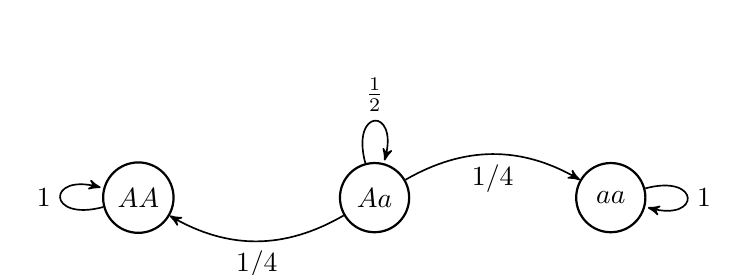
\begin{tikzpicture}[->, >=stealth', auto, semithick, node distance=3cm]
	\tikzstyle{every state}=[fill=white,draw=black,thick,text=black,scale=1]
	\node[state]    (A)                     {$AA$};
	\node[state]    (B)[right of=A]   {$Aa$};
	\node[state]    (C)[right of=B]   {$aa$};
	\path
	(A) edge[loop left]			node{$1$}	(A)
	(B) edge[bend left,below]	node{$1/4$}	(A)
	(B) edge[loop above]		node{$\frac{1}{2}$}	(B)
	(B) edge[bend left,below]	node{$1/4$}	(C)
	(C) edge[loop right]		node{$1$}	(C);
	%\node[above=0.5cm] (A){Patch G};
	%\draw[red] ($(D)+(-1.5,0)$) ellipse (2cm and 3.5cm)node[yshift=3cm]{Patch H};
	\end{tikzpicture}
\end{center}
Det er derudover muligt at lave overgangsmatricen hvor $p_{ij}$ er indgang $i,j$. 
\begin{align*}
    P=
\begin{bmatrix}
1 & 0 & 0 \\
\frac{1}{4} & \frac{1}{2} & \frac{1}{4}\\
0 & 0 & 1
\end{bmatrix}
\end{align*}
\end{eks}

\subsection{Tidsdynamik af Markov-kæder}
Det er muligt at analysere hvordan Markov-kæder udvikler sig over tid. Det er muligt ud fra kendte sandsynligheder at beregne fremtidige sandsynligheder. Overgangsmatricen består af $p_{ij}$ som er \textit{et-trins overgangssandsynligheder}, hvor man generelt kan skrive \textit{n'te-trins overgangssandsynligheder} som 
\begin{align*}
    p_{ij}^{(n)} = P ( X_n = j | X_0 = i)
\end{align*}
Hvorom det gælder at den n'te-trins overgangsmatrice er $P^{(n)}$. Denne matrice opfylder følgende

\begin{minipage}\textwidth
\begin{thmx} \textbf{Chapman-Kolmogorov ligningen}\label{sæt:chapman-kolmogrov} %Ny sætning
\newline
Det gælder at 
\begin{align*}
    p_{ij}^{(n+m)} = \sum_{k \in S} p_{ik}^{(n)}p_{kj}^{(m)}
\end{align*}
for alle $m,n$ og alle $i,j \in S$. Altså gælder $P^{(n+m)} = P^{(n)}P^{(m)} = P^{n}P^{m}$.
\end{thmx}
\end{minipage}

\begin{bev} \textbf{} %Nyt bevis
\newline
Ud fra Loven om total sandsynlighed, \autoref{sæt:loven_om_total_sandsynlighed}, gælder det at
\begin{align*}
    p_{ij}^{(n+m)} &= P(X_{n+m} = j | X_0 = i) = \sum_{k \in S} P (X_{n+m} = j | X_n = k, X_0 = i)P(X_n=k|X_0=i)
    \intertext{Af Markov egenskaben får dermed at}
    p_{ij}^{(n+m)} &=\sum_{k \in S} P (X_{n+m} = j | X_n = k, X_0 = i)P(X_n=k|X_0=i) \\
    &= \sum_{k \in S} P (X_{n+m} = j | X_n = k)P(X_n=k|X_0=i) \\ 
    &= \sum_{k \in S} p_{ik}p_{kj}
\end{align*}
Dermed er \autoref{sæt:chapman-kolmogrov} bevist.
\end{bev}
Når $P^{(n)}$ er bestemt er det muligt bestemme Markov-kædens langsigtet adfærd. Dette gøres ved at bestemme
\begin{align*}
    \lim_{n \to \infty} P^{(n)}
\end{align*}
Hvis de asymptotiske sandsynligheder ikke afhænger af \textbf{?begyndelsestilstanden?} kaldes fordelingen på det givne tilstandsrum for en \textbf{\textit{grænsefordelling}}.

\subsection{Klassifikation af tilstande}
Når Markov-kæder skal analyseres, er en vigtig del at se på om tilstande kan "nå" hinanden eller ej. Derfor defineres følgende.\\
\begin{minipage}\textwidth
\begin{defn}\textbf{Tilgængelighed} \label{def:tilgængelighed} %Ny definition
\newline
Hvis $p_{ij}^{(n)}>0$ for et givent $n$, siges tilstanden, $j$, at være \textit{tilgængeligt} fra tilstanden $i$. Dette noteres, $i\to j$. Hvis $i\to j$ og $j\to i$, siges det, at $i$ og $j$ \textit{kommunikerer}, hvilket noteres $i\leftrightarrow j$. 
\end{defn}
\end{minipage}

Hvis en tilstand, $i \in S$, kun kommunikerer med én tilstand, $j \in S$, danner disse en \textit{kommunikerende klasse}. Det er muligt at alle tilstande i $S$ kommunikerer med hinanden, hvilket fører til følgende definition
 
\begin{minipage}\textwidth
\begin{defn}\textbf{} %Ny definition
\newline
Hvis alle tilstande i $S$ kommunikerer med hinanden, siges Markov-kæden at være $ureducerbar$.
\end{defn}
\end{minipage}

Ud over at det er vigtigt at vide om tilstande kommunikerer er det også vigtigt at vide om man vender tilbage til en tilstand. I følgende definition klassificeres tilstande i forhold til om det er sikkert at man vender tilbage til den. 

\begin{minipage}\textwidth
\begin{defn}\textbf{} %Ny definition
\newline
Lad $i\in S$ være en tilstand, $\tau_i$ være antallet af skridt før kæden besøger $i$ og $P_i$ være sandsynlighedsfordellingen for kæden i begyndelsestilstanden $X_0=i$. Altså
\begin{align*}
    \tau_i=min\{n\geq1:X_n=i\}
\end{align*}
hvor $\tau_i=\infty$ hvis $i$ aldrig bliver besøgt. Hvis $P_i(\tau_i<\infty)=1$, siges tilstanden $i$ at være \textit{tilbagevendende}. Hvis den ikke er tilbagevendende, siges den at være  \textit{forbigående}.
\end{defn}
\end{minipage}

Altså gælder det at hvis en tilstand er tilbagevendende vil Markov-kæden med sikkerhed vende tilbage til tilstanden. Hvis tilstanden derimod er forbigående vil der være en sandsynlighed for, at Markov-kæden ikke vender tilbage til tilstanden. For ureducerbare Markov-kæder gælder følgende

\begin{minipage}\textwidth
\begin{kor} \textbf{} \label{kor:enten_forbigå_eller_tilbagevend}%Nyt k
\newline
I en ureducerbar Markov-kæde er alle tilstande enten forbigående eller tilbagevendende.
\end{kor}
\end{minipage}

\begin{bev} \textbf{} %Nyt bevis
\newline
Da Markov-kæden er ureducerbar gælder det at $i \leftrightarrow j$ for alle $i,j \in S$. Af \autoref{def:tilgængelighed} gælder det da at $i \to j$ og $j \to i$, og dermed eksisterer der $n,m$ således at
\begin{align*}
    p_{ij}^{(n)} > 0 \quad \text{ og } \quad p_{ji}^{(m)} > 0
\end{align*}

\end{bev}

Det er herved muligt at konkluderer at alle tilstande er tilbagevendende eller forbigående hvis dette gælder for én tilstand. For et endeligt tilstandsrum er der givet følgende korollar

\begin{minipage}\textwidth
\begin{kor} \textbf{} \label{kor:forbigående}%Nyt korollar
\newline
Lad S være endelig. En tilstand siges at være forbigående hvis og kun hvis der eksisterer en anden tilstand j således at $i \to j$ men $j \not\to i.$
\end{kor}
\end{minipage}

%Af \autoref{kor:forbigående} fremgår det, at når en Markov-kæde går gennem en forbigående tilstand, er der en sandsynlighed for, at kæden ikke vil gå tilbage igen.

I et endeligt tilstandrum er det kun muligt for en Markov-kæde at være forbigående, hvis der er endnu en tilstand, der kan nåes, men som ikke har en rute tilbage. I en uendeligt tilstandsrum er det muligt, at der kun er forbigående tilstande, selvom de alle er kommunikerende. 

For at bevise Proposition \ref{tilbagevendende}, introduceres følgende genererende funktioner. Lad $i,j\in S$ og
$$p_{ij}=\sum_{n=0}^\infty p_{ij}(n)s^n, \quad F_{ij}(s)=\sum_{n=0}^\infty p_i(\tau_j=n)s^n$$
Med konventionerne, $p_i(\tau_j=0)=0$ og $p_{ij}(0)=\delta_{ij}$ følger det, at \textit{Kronecker} deltaet defineres som
\begin{align*}
    \delta_{ij}=\begin{cases}1\ \text{hvis } i=j,\\0\ ellers\end{cases}
\end{align*}


\begin{lem}\label{overgangssandynlighed Kronecker}
For $i,j\in S$ gælder, at
\begin{align*}
    p_{ij}(s)=\delta_{ij}+F_{ij}(s)p_{jj}(s),\quad s\in(-1,1]
\end{align*}
\end{lem}

\begin{bev} %Nyt bevis
Ved at betinge værdien af $\tau_j$,
gælder ifølge Loven om Total Sandsynlighed, at
\begin{align}\label{tau_j betinget}
    p_{ij}(n)=\sum_{m=1}^\infty p_i(X_n=j|\tau_j=m)p_i(\tau_j=m), \quad n\geq 1
\end{align}
hvor $X_n$ er betinget af $\tau_j$.
Summanden er $0$ for $m>n$, eftersom det første besøg til $j$ ikke har sket tiden $n$. For $m\leq n$ gælder, at
\begin{align*}
    p_i(X_n=j|\tau_j=m)=p_i(X_n=j|X_m=j, H)
\end{align*}
hvor $H=\{X_r\neq j \text{ for } 1\leq r <m\}$ er en hændelse defineret før tiden $m$.
Det følger af antagelsen om homogenitet og den udvidede Markov egenskab, at
\begin{align*}
    p_i(X_n=j|\tau_j=m)=p(X_n=j|X_m=j)=p_j(X_{n-m}=j)
\end{align*}
Ved at indsætte dette i \eqref{tau_j betinget} fås
\begin{align*}
    p_{ij}(n)=\sum_{m=1}^n p_{jj}(n-m)p_i(\tau_j=m), \quad n\geq 1
\end{align*}
Ved at multiplicere ligningen med $s^n$ og summe over $n\geq 1$ fås
\begin{align*}
    p_{ij}(s)-p_{ij}(0)=p_{jj}(s)F_{ij}(s)
\end{align*}
Dette beviser sætningen, eftersom $p_{ij}(0)=\delta_{ij}$.
\end{bev}

\begin{minipage}\textwidth
\begin{thmx}\label{tilbagevendende} \textbf{} %Ny proposition
\newline
Tilstanden, $i$ er tilbagevendende, hvis
\begin{align*}
 \sum_{n=1}^\infty p_{ii}^{(n)}=\infty
\end{align*}
\end{thmx}
\end{minipage}
\begin{bev}
Hvis $i=j$ følger det af \eqref{overgangssandynlighed Kronecker}, at
\begin{align}\label{i=j}
    p_{ii}(s)=\frac{1}{1-F_{ii}(s)} \text{ for } |s|<1
\end{align}
Der gælder ifølge Abel's lemma, at
\begin{align*}
    F_{ii}(s)\uparrow F_{ii}(1), \quad p_{ii}\uparrow\sum_{n=0}^\infty p_{ii}(n)
\end{align*}
Det følger af \eqref{i=j}, at
\begin{align*}
    \sum_{n=0}^\infty p_{ii}(n)=\infty \text{ hvis og kun hvis } F_{ii}(1)=1
\end{align*}

\end{bev}

\subsection{Stationære distributioner}


\begin{minipage}\textwidth
\begin{defn}\textbf{} %Ny definition
\newline
Lad $P$ være en overgangsmatrice for en Markov-kæde med tilstandsrummet, $S$. En sandsynlighedsdistribution, $\bm\pi=(\pi_1,\pi_2,\dots)$ på $S$, som opfylder
\begin{align*}
    \bm\pi P=\bm\pi
\end{align*}
kaldes for en \textit{stationær distribution} på kæden. 
\end{defn}
\end{minipage}

Indgangene i $\pi$ må dermed opfylde, at
\begin{align*}
    \pi_j=\sum_{i\in S}=p_{ij}\pi_i \text{ for alle } j\in S
\end{align*}
hvilket med betingelsen:
\begin{align*}
    \sum_{i\in S} \pi_i=1
\end{align*}
bestemmer den stationære distribution. 



\chapter{Markov beslutningsprocesser}
%https://onlinelibrary-wiley-com.zorac.aub.aau.dk/doi/pdf/10.1002/9780470316887
Dette kapitel er baseret på \cite[s. 17-25, 78-91 og 143-146]{"Markov_decision_process"}.

I dette kapitel redegøres for de processer, der opfylder markovegenskaben. Disse kaldes for \textit{Markov beslutningsprocesser}. 

\section{Beslutningsmodel}
For at beskrive Markov beslutningsprocesser introduceres begrebet beslutningsmodel. De centrale begreber for en beslutningsmodel er følgende  
\begin{enumerate}
    \item Beslutningstager
    \item Beslutningstidspunkt
    \item Tilstande
    \item Beslutninger
    \item Belønninger eller omkostninger som følge af en beslutning % (vi skriver kun belønninger, omkostninger er implicit)
\end{enumerate}
Til et specifik beslutningstidspunkt observerer en beslutningstager en tilstand i et system. Ud fra denne observation tager beslutningstageren en beslutning. Denne beslutning resulterer i, at beslutningstageren får en belønning eller omkostning, og systemet udvikler sig til en ny tilstand til det efterfølgende beslutningstidspunkt. Ved denne nye tilstand skal beslutningstageren tage en ny beslutning, som fører til en ny tilstand. Denne proces fortsætter, hvoraf beslutningstageren modtager en sekvens af belønninger og omkostninger. For beslutningstageren er målet at optimere belønningerne og minimere omkostningerne.

%Problem -- beslutninger, tilstande -- beslutningstager --taget en beslutning-- reward/cost

\section{Markov beslutningsprocesser}\label{afsnit:Markov_beslutningsprocesser}
En Markov beslutningsproces er en beslutningsmodel, og er dermed baseret på begreberne beslutninger, heriblandt beslutningstager og beslutningstidspunkter, samt tilstande og belønninger. For en Markov beslutningsproces afhænger tilstande til fremtidige beslutningstidspunkter af den nuværende tilstand og de forrige beslutninger. Beslutningstageren skal derfor ikke udelukkende tage beslutninger ud fra kortsigtede belønninger, men også ud fra de fremtidige for at kunne optimere sine belønninger. 


%En beslutningstager kan påvirke et probabilistisk system over tid. Målet er at vælge en sekvens af hændelser / beslutninger, som får systemet til at fungere optimalt i forhold til et vis kriterie. Tilstanden af systemet i morgen afhænger af tilstanden i dag, samt beslutningen i dag. Man bliver dermed nødt til at tænke frem og man skal forudse mulighederne og omkostningerne (eller belønninger) forbundet med fremtidige systemtilstande. 


\subsection{Beslutningstidspunkter}
I \autoref{Kap:MArkov-kæder} er hver tilstand indekseret af et indeks i mængden $T$, som kaldes for indeksmængden. For en Markov beslutningsproces består denne indeksmængde af diskrete beslutningstidspunkter, $t$. Mængden af beslutningstidspunkter er enten endelig eller uendelig. %Der gælder, at $T$ er en endelig eller uendelig mængde af diskrete beslutningstidspunkter $t$.%, hvor hvert element i $T$ noteres $t$.

%$T$ er mængden af beslutningstidspunkter. Beslutningstidspunkterne tager udgangspunkt i diskret tid med tilfældige tidsperioder, hvor forskellige begivenheder optræder. Eksempelvis ved et køsystem eller ved tidspunkter valgt af beslutningstageren. Denne tid er opdelt i perioder eller tilstande. Beslutningstidspunkter er enten endelige, uendelige, eller begrænset i intervaller.

\subsection{Tilstande og beslutninger}
Til ethvert beslutningstidspunkt, $t$, er systemet i en tilstand. Mængden af mulige tilstande i systemet betegnes $S$ og lad $s\in S$ være en tilstand. Tilstandsrummet, $S_t$, er mængden af mulige tilstande i systemet til beslutningstidspunktet, $t$. 

Mængden af mulige beslutninger ved tilstanden, $s$, kaldes beslutningsrummet og noteres $A_s$. Det noteres $A_{s,t}$, hvis beslutningerne også afhænger af $t$. Hver enkelte beslutning betegnes $a$. Beslutninger kan enten tages tilfældigt eller deterministisk. Hvis hver beslutning tages tilfældigt, betyder det, at de tages med en bestemt sandsynlighed. Hvis beslutningerne derimod vælges deterministisk, vil sandsynligheden for én beslutning være 1, mens den for alle andre vil være 0.


%Lad $(\Omega, \F, P)$ være et sandsynlighedsrum. 
Det gælder, at $S_t$ og $A_{s,t}$ er diskrete og tællelige mængder. Det bemærkes, at \\$S=\displaystyle \bigcup_{t\in T}S_t$ og $A_s=\displaystyle\bigcup_{t\in T}A_{s,t}$ og .


%Lad $S_t$ angive mængden af mulige tilstande til tiden $t$, sådan at $S=\bigcup_{t\in T} S_t$ og lad $A_{s,t}$ være mængden af tilladte hændelser i tilstand $s\in S$ og tid $t$. Så er $A_s=\bigcup_{t\in T} A_{s,t}$ og beslutningstageren kan i så fald vælge enhver hændelse, $a\in A_s$. Lad $A=\bigcup_{s\in S} A_s$. Hændelser kan enten vælges tilfældigt eller deterministisk. Lad $P(A_s)$ angive mængden af sandsynligshedsfordelinger for delmængder af $A_s$ og ligeledes, $P(A)$ være sandsynlighedsfordelinger på delmængder af $A$.

\subsection{Belønningssandsynlighed}
Når beslutningstageren har taget en beslutning, $a\in A_{s}$ til beslutningstidspunktet, $t$, vil beslutningstageren modtage en belønning, $r_t(s,a)$. Hvis $r_t(s,a)$ er negativ, vil beslutningen resultere i en omkostning. Hvis belønningen er afhængig af tilstanden til næste beslutningstidspunkt, betegnes belønningen $r_t(s, a, s')$, hvor $s'$ er tilstanden til beslutningstidspunktet, $t+1$.
Når beslutningen er taget, vil tilstanden til næste beslutningstidspunkt blive bestemt ved sandsynlighedsfordelingen, $p_t(\cdot|s,a)$. 


% For at gøre rede for belønningen ved et tilfældigt eksperiment, vil handlingen beskrives ved $a \in A_s$, i et stadie, $s$, til beslutningstidspunkt, $t$.
% Denne belønning beskrives ved $r_t(s,a)$. Tilstanden ved næste beslutningstidspunkt er afhængig af sandsynlighedsfordelingen, $p_t(\cdot|s,a)$.

%Denne belønning kan beskrives ved $r_t(s,a)$, hvoraf den næste beslutning er givet ved sandsynligheden $p_t(\cdot | s,a)$.\\
%Desuden bemærkes det, at en negativrt(s,a)vil belønningen være en udgift. Når belønnin-gen afhænger af systemets tilstand til den næste beslutningsperiode, kan r_t(s,a,j)beskrive
% værdien til tiden t af belønningen, og hvor j beskriver et stadie i beslutningsperioden til t+ 1.

%Desuden bemærkes det, at hvis $r_t(s,a)$ er negativ, vil belønningen være en udgift. 
%Når belønningen afhænger af systemets tilstand ved næste beslutningstidspunkt, beskriver $r_t(s,a,j)$ belønningen til tiden $t$, hvor $j$ er tilstanden til beslutningstidspunktet, $t+1$.

Den forventede værdi til beslutningstidspunktet, $t$, kan beregnes ved 
\begin{align*}
    r_t(s,a)=\sum_{s'\in S} r_t(s,a,s')p_t(s' | s,a),
\end{align*}
%
% Følgende definition beskriver den forventede værdi af belønningen til beslutningstidspunktet, $t$.
% \begin{defn}
%  \textbf{Forventet værdi af belønning}
% \newline
% Lad $s$ være en tilstand i tilstandsrummet $S$ og $a$ være en beslutning i beslutningsrummet $A_s$. Lad $r_t$ være belønningen og $p_t$ være sandsynligheden.
% %Lad $p_t(j | s,a)$ være en ikke-negativ funktion
% Den forventede værdi af belønningen til beslutningstidspunktet $t$ er givet ved
% \begin{align*}
%     r_t(s,a)=\sum_{s'\in S} r_t(s,a,s')p_t(s' | s,a),
% \end{align*}
% hvor $s' \in S$ er tilstanden til beslutningstidspunktet $t+1$.
%
% \end{defn}
%
%Funktionen $p_t(j |s,a)$ beskriver sandsynligheden for, at systemet er i tilstand $j \in S$ til tiden $t+1$, når valget, $a \in A$, er givet. 
%p: S \to [0,1]
%
Funktionen, $p_t(s'|s,a)$, kaldes overgangssandsynlighedsfunktionen, hvor $\displaystyle\sum_{s'\in S} p_t(s'|s,a)=1$.


For en Markov beslutningsproces med en endelig indeksmængde, $T$, gælder det, at der ikke tages en beslutning til det sidste beslutningstidspunkt, $N$. Derfor er belønningen til beslutningstidspunktet, $N$, kun en funktion af tilstanden og betegnes $r_N(s)$.

Ud fra ovenstående siges følgende mængde at være en Markov beslutningsproces
%
\begin{align*}
    \left(T, S, A_s, p_t(\cdot | s,a), r_t(s,a)\right).
 \end{align*}
 %
Dette er en Markov beslutningsproces, da overgangssandsynligheden og belønningen kun afhænger af det forrige beslutningstidspunkt. 



%Hvis Markov beslutningsprocessen har en endelig horisont, er der ikke givet nogen beslutning ved beslutningstiden, $N$. Til denne tid er belønningen, $r_N(s)$, udelukkende en funktion af tilstanden og kaldes for \textit{nyværdien}.
% %En Markov beslutningsproces er en mængde af objekter, givet ved:
% \begin{align*}
%     \{T, S, A_s, p_t(\cdot | s,a), r_t(s,a)\}.
% \end{align*}

% Det skyldes nemlig, at overgangssandsynligheden og belønningsfunktionen afhænger af den forrige tilstand og beslutningen taget i denne tilstand.



%decision rule?
\subsection{Beslutningsregel}\label{afsnit:beslutningsregel}
En beslutningsregel er en procedure til at vælge beslutninger for hver tilstand til et givet beslutningstidspunkt, $t$. Beslutningsregler kan både være deterministiske og tilfældige.% men i dette projekt tages der udgangspunkt i deterministiske beslutningsregler.

En deterministisk beslutningsregel er en funktion, $d_t:S\to A_s$, som angiver beslutningsvalget ved tilstanden, $s$, og beslutningstidspunkt, $t$. Beslutningsreglen siges at være Markov, hvis den kun afhænger af de forrige tilstande og beslutninger gennem den nuværende tilstand af systemet. 

En deterministisk beslutningsregel kan være fortidsafhængig, hvis den afhænger af en historik. En historik er en ordnet mængde af skiftevis tilstande og beslutninger, $h_t = (s_1, a_1, \dots,  s_{t-1}, a_{t-1}, s_t)$, som følger rekursionen, $h_t=(h_{t-1}, a_{t-1}, s_t)$. En deterministisk beslutningsregel er fortidsafhængig, hvis den afhænger af den forrige historik, $h_t$.
Lad $H_t$ angive mængden af alle historikker, $h_t$. Bemærk, at 
\begin{align*}
    H_1&=S, \quad H_2=S\times A\times S, \quad H_n =S\times A\times S\times \cdots \times S \text{ og }\\
    H_t&=H_{t-1}\times A\times S. 
\end{align*}
En fortidsafhængig deterministisk beslutningsregel er en funktion, $d_t: H_t\to A$, under betingelsen, at $d_t(h_t)\in A_{s_t}$.

En tilfældig beslutningsregel, $d_t$, er en funktion, $d_t: S\to P(A)$, som angiver sandsynligheden for en beslutning ved tilstanden, $s$, til beslutningstidspunktet, $t$. Altså angiver en tilfældig beslutningsregel sandsynlighedsfordelingen, $q_{d_t}(\cdot)$, for mængden af beslutninger til beslutningstidspunktet, $t$. For en fortidsafhængig tilfældig beslutningsregel, gælder det, at $d_t:H_t\to P(A)$.

Når den tilfældige beslutningsregel er Markov, er $q_{d_t(s_t)}\in P(A_{s_t})$. Hvis den tilfældige beslutningsregel derimod er fortidsafhængig, vil $q_{d_t(h_t)}\in P(A_{s_t})$ for alle $h_t\in H_t$.

En deterministisk beslutningsregel er et specialtilfælde af en tilfældig beslutningsregel, hvor 
\begin{align*}
    q_{d_t(s_t)}(a)=1,\\
    q_{d_t(h_t)}(a)=1
\end{align*}
for ét $a\in A_s$. Mængden af alle beslutningsregler betegnes ved $D_t^K$, hvor $K$ er klassen af beslutningsregler. Der er fire forskellige klasser, som er gennemgået ovenfor Markov deterministisk (MD), fortidsafhængig deterministisk (FD), Markov tilfældig (MT) og fortidsafhængig tilfældig (FT). 

\subsection{Strategi}
En strategi er en sekvens af beslutningsregler $\Psi=(d_1,d_2,\dots,d_{N-1})$, hvor $d_t\in D_t^K$ for alle $t=1, 2, \dots N-1$ for $N \leq \infty$. Altså indeholder en strategi den beslutningsregel, der skal anvendes til ethvert beslutningstidspunkt, og dermed ved beslutningstageren, hvilken beslutning der skal vælges til enhver tilstand. En strategi er invariant, hvis $d_t=d$ for alle $t\in T$. Dette har formen, $\Psi=(d,d,\dots)$ og betegnes ved $d^\infty$. 
Mængden af alle strategier for $K=MD, FD, MT, FT$ betegnes $\Pi^K=D_1^K\times D_2^K\times \cdots\times D_{N-1}^K$.

% En \textit{strategi} bestemmer hvilke beslutningsregler, der skal benyttes til ethvert beslutningstidspunkt. Med andre ord er det en sekvens/følge af beslutningsregler, $\Psi=(d_1,d_2,\dots,d_{N-1})$, hvor $d_t\in D_t^k$.
% Lad nu $\Pi=D_1\times D_2,\times\cdots\times D_{n-1}, N\leq \infty$ være en endelig eller uendelig mængde af alle strategier.

% En strategi er invariant, hvis $d_t=d$ for alle $t\in T$. Dette har formen, $\pi=(d,d,\dots)$ og betegnes ved $d^\infty$. 

\section{Induceret stokastisk proces, betingede sandsynligheder og forventede værdier og et andet navn}

% Symbolerne for sandsynlighedsrum, hændelsesrum og lignende anvendes uden forklaring i følgende afsnit.

%Symbolerne som er præsenteret i underafsnit \ref{afsnit:Markov_beslutningsprocesser} anvendes uden forklaring i det resterende af dette kapitel, og derfor præsenteres de ikke i resultaterne i de følgende underafsnit. 

Af \autoref{def:sandsynlighedsrum} gælder det, at et sandsynlighedsrum er givet ved triplen, $(\Omega, \F, P)$, hvor $\Omega$ betegner udfaldsrummet, $\F$ hændelsesrummet og $P$ et sandsynlighedsmål på $(\Omega,\mathcal{F})$. I dette afsnit er $\F$ potensmængden af $\Omega$.

Udfaldsrummet er givet ved
\begin{align*}
    \Omega = S \times A \times S \times \cdots \times S = \{S \times A\}^{N-1} \times S
\end{align*}
for en endelig indeksmængde $T=\{1, 2,\cdots, N\}$, hvor $N<\infty$, og
\begin{align*}
    \Omega = \{S \times A\}^\infty
\end{align*}
for en uendelig indeksmængde, hvor $N=\infty$.

% For en endelig indeksmængde, $T=\{1, 2,\cdots, N\}$, hvor $N<\infty$, så er udfaldsrummet givet ved gælder det, at
% \begin{align*}
%     \Omega = S \times A \times S \times \cdots \times S = \{S \times A\}^{N-1} \times S,
% \end{align*}
% og for en uendelig indeksmængde, hvor $N=\infty$, er 
% \begin{align*}
%     \Omega = \{S \times A\}^\infty.
% \end{align*}
Hvert element $\omega \in \Omega$ kaldes en \textit{udfaldsvej} og består af en sekvens af tilstande og beslutninger. Altså
\begin{align*}
    \omega=(s_1 , a_1 , s_2 , a_2 , \dots , a_{N-1} , s_N).
\end{align*}
Hvis $N<\infty$, er indeksmængden endelig, og hvis $N=\infty$, er indeksmængden uendelig. 
Lad $X_t$ og $Y_t$ være to tilfældige variabler, som er givet ved
\begin{align*}
    X_t(\omega) = s_t \text{ og } Y_t(\omega) = a_t \text{ for } t=1,2,\dots, N, \  N\leq \infty,
\end{align*}
hvor $X_t$ antager værdier i tilstandsrummet, $S$, og $Y_t$ antager værdier i beslutningsrummet, $A$. Altså gælder det, at $X_t$ betegner tilstanden til $t$ og $Y_t$ betegner beslutningen til $t$ for en udfaldsvej, $\omega$.

Lad derudover $Z_t$ være en tilfældig variabel, som er givet ved
\begin{align*}
    Z_1(\omega) = s_1 \text{ og } Z_t(\omega) = (s_1 , a_1 , s_2 , a_2 , \dots , s_t) \text{ for } t=1,2, \dots, N, \  N\leq \infty.
\end{align*}

En fortidsafhængig strategi $\Psi = (d_1, d_2, \dots, d_{N-1})$, hvor $N \leq \infty$, inducerer en sandsynlighed, $P^\Psi$, på $(\Omega, \F)$ ved
\begin{align}
    P^{\Psi}(X_1=s)&=P_1(s)\label{eqs:de_tre_ligninger},\\
    P^{\Psi}\left(Y_t=a|Z_t=h_t\right)&= q_{d_t(h_t)}(a)\label{eqs:de_tre_ligninger2},\\
    P^{\Psi}\big(X_{t+1}=s|Z_t&=(h_{t-1}, a_{t-1}, s_t), Y_t=a_t \big)=p_t(s|s_t, a_t), \label{eqs:de_tre_ligninger3}
\end{align}
hvor $P_1(s)$ betegner begyndelsesfordelingen til tilstanden $s$.

Af kædereglen for sandsynligheder, (se \autoref{bilag:kædereglen}), følger det, at sandsynligheden for en udfaldsvej, $\omega =(s_1 , a_1 , s_2 , \dots , a_{N-1} , s_N)$, er givet ved
\begin{align}
    P^\Psi(s_1 , a_1 , s_2 , \dots , s_N) &= P(s_1)P(a_1|s_1)P(s_2|a_1 , s_1)P(a_2|s_2 , a_1 , s_1)\nonumber \\
    &\phantom{= \ }\cdots P(a_{N-1}|s_{N-1} , \dots , a_1 , s_1) P(s_N | a_{N-1} , \dots , a_1 , s_1).\nonumber
    % \intertext{Af Markov egenskaben, \autoref{markov-kæde-hovedsætning}, gælder det, at}
    % P^\Psi(s_1 , a_1 , s_2 , \dots , s_N) &= P(s_1)P(a_1|s_1)P(s_2|a_1 , s_1)P(a_2|s_2 , a_1 , s_1)\nonumber \\
    % &\phantom{= \ }\cdots P(a_{N-1}|s_{N-1} , a_{N-2}) P(s_N | a_{N-1} , s_{N-1}).\nonumber
    \intertext{Ved at anvende \eqref{eqs:de_tre_ligninger2} og \eqref{eqs:de_tre_ligninger3} fås}
    P^\Psi(s_1 , a_1 , s_2 , \dots , s_N) &= P(s_1)q_{d_1(s_1)}(a_1)p_1(s_2|s_1 , a_1)q_{d_2(h_2)}(a_2)\nonumber\\
     &\phantom{= \ }\cdots q_{d_{N-1}(h_{N-1})}(a_{N-1})p_{N-1}(s_N|a_{N-1} , s_{N-1}).\label{eq:den_meget lange_der_er_træls_at_skrive}
\end{align}
Fra \autoref{afsnit:beslutningsregel} vides det, at når en strategi, $\Psi$, er deterministisk, eksisterer der et $a\in A_s$ således, at $q_{d_t(s_t)}(a) = 1$ og $q_{d_t(h_t)}(a)=1$. Dermed gælder det for en deterministisk strategi, $\Psi$, at
\begin{align*}
    P^\Psi(s_1 , a_1 , s_2 , \dots , s_N) &= P(s_1)p_1(s_2|s_1 , a_1)\cdots p_{N-1}(s_N|a_{N-1} , s_{N-1}).
\end{align*}
De ovenstående ligninger skal anvendes til at bestemme udtrykket for følgende betingede sandsynlighed 
\begin{align}
    P^\Psi(a_t , s_{t+1}, \dots, s_N | s_1 , a_1 , \dots , s_t) = \frac{P^\Psi(s_1 , a_1 , \dots , s_N)}{P^\Psi(s_1 , a_1 , \dots , s_t)}, \label{eq:betinget_sands_for_meget_lang_udtryk}
\end{align}
som følger af kædereglen for sandsynligheder, (se \autoref{bilag:kædereglen}), for $P^\Psi(s_1 , a_1 , \dots , s_t) \neq 0$. Bemærk, at \\
$ P^\Psi(a_t , s_{t+1}, \dots, s_N | s_1 , a_1 , \dots , s_t) = 0 $, hvis $P^\Psi(s_1 , a_1 , \dots , s_t) = 0$.

% under antagelsen af, at $P^\Psi(s_1 , a_1 , \dots , s_t) \neq 0$.

Ved at sætte $N=t$ i \eqref{eq:den_meget lange_der_er_træls_at_skrive} vides det, at 
\begin{align*}
    P^\Psi(s_1 , a_1 , s_2 , \dots , s_t) &= P(s_1)q_{d_1(s_1)}(a_1)p_1(s_2|s_1 , a_1)q_{d_2(h_2)}(a_2)\\
     &\phantom{= \ }\cdots q_{d_{t-1}(h_{t-1})}(a_{t-1})p_{t-1}(s_t|a_{t-1} , s_{t-1}).
\end{align*}

Udtrykkene i brøken for \eqref{eq:betinget_sands_for_meget_lang_udtryk} indsættes og reduceres
\begin{align*}
P^\Psi(a_t , s_{t+1}, \dots, s_N | s_1 , a_1 , \dots , s_t) &=\frac{P(s_1)q_{d_1(s_1)}(a_1)
    \cdots p_{N-1}(s_N|a_{N-1} , s_{N-1})}{P(s_1)q_{d_1(s_1)}(a_1)
    \cdots p_{t-1}(s_t|a_{t-1} , s_{t-1})}\\
    &= q_{d_t(h_t)}(a_t)p(s_{t+1}|s_t , a_t)\\
    &\phantom{= \ } \cdots q_{d_{N-1}(h_{N-1})}(a_{N-1})p_{N-1}(s_N|s_{N-1} , a_{N-1}).
\end{align*}
Hvis en strategi, $\Psi$, er Markov, så afhænger beslutningsreglen, $d_t$, kun af de forrige tilstande og beslutninger gennem den nuværende tilstand. Det gælder altså, at 
\begin{align*}
    q_{d_t(h_t)}(a)= P^\Psi \left(Y_t = a | Z_t = (h_{t-1} , a_{t-1} , s_t) \right) = P \left(Y_t = a | X_t = s_t\right) = q_{d_t(s_t)}(a).
\end{align*}
Dermed følger det, at
\begin{align*}
    P^{\Psi}\left(a_t , s_{t+1} , \cdots , s_N|s_1 , a_1 , \cdots , s_t\right)=P^{\Psi}\left(a_t , s_{t+1} , \cdots , s_N|s_t\right).
\end{align*}

\subsection{Markov belønningsproces}
En Markov belønningsproces er den bivariate stokastiske proces $\left\{\left(X_t, r_t(X_t, Y_t)\right); t \in T\right\}$, når en strategi, $\Psi$, er Markov. Denne stokastiske proces består af en sekvens af tilstande og belønninger givet en strategi, $\Psi$. 

Lad $W$ være en diskret tilfældig variabel defineret på sandsynlighedsrummet, $(\Omega, \F, P^{\Psi})$, hvor
\begin{align*}
    W(\omega)=W(s_1 , a_1 , \dots , s_N) = \sum_{t=1}^{N-1} r_t(s_t,a_t) + r_N(s_N).
\end{align*}
Dermed er $W(\omega)$ summen af belønninger. Af \autoref{def:Forventetværdi} følger det, at
\begin{align*}
    E^\Psi [W] = \sum_{\omega \in \Omega} W(\omega)P^\Psi\left(\omega\right) = \sum_{w \in Range(W)} w P^\Psi \left(w: W(\omega) = w\right), 
\end{align*}
hvor $E^\Psi(W)$ betegner den forventede værdi til $W$ givet strategien $\Psi$. Hvis Omega ikke er tællelig, bliver summerne i ovenstående til integraler. 
 %Summerne i ovenstående bliver til integraler for $N = \infty$ og $E^\Psi(W)$ betegner den forventede værdi til $W$ givet strategien $\Psi$.

Hvis strategien $\Psi$ er fortidsafhængig med historikken $h_t=(s_1, a_1 , \dots , s_t)$, og $W$ er en funktion af $s_t, a_t,\dots, s_N$, så gælder det, at
\begin{align}\label{eq:forventet_belønning_fortidsafhængig}
    E_{h_t}^\Psi \left[W(X_t , Y_t , \dots , X_N) \right] = \sum W(s_t , a_t , \dots , s_N) P^\Psi (a_t , s_{t+1} , \dots , s_N | s_1 , a_1 , \dots , s_t),
\end{align}
hvor der summes over $(a_t , s_{t+1} , \dots , s_N) \in A \times S \times \cdots \times S$. Er strategien, $\Psi$, derimod Markov, følger det, at
\begin{align*}
     E_{s_t}^\Psi \left[W(X_t , Y_t , \dots , X_N) \right] = \sum W(s_t , a_t , \dots , s_N) P^\Psi (a_t , s_{t+1} , \dots , s_N | s_t).
\end{align*}

%For en beslutningstager gælder det om at optimere denne sum, så der opnås størst mulig belønning.   
% \subsection{Markov modellen}

% I dette afsnit konstrueres en model for den stokastiske model genereret ud fra Markov beslutningsprocessen. Det antages, at $S$ og $A$ er diskrete.

% Som nævnt i sandsynlighedsafsnittet, består et sandsynlighedsrum af tre elementer: et udfaldsrum, $\Omega$, et hændelsesrum, $\mathcal{F}$ og et sandsynlighedsmål, $P$, på $(\Omega,\mathcal{F})$.
% Bemærk, at når $\Omega$ er endelig, så er $\mathcal{F}$ givet ved potensmængden af $\Omega$ og sandsynlighedsmålet er en sandsynlighedsmassefunktion. 

% For en MDP med endelig horisont, vælges
% \begin{align*}
%     \Omega=S\times A\times S\times A\times\cdots\times A\times S=\{S\times A\}^{N-1}\times S,
% \end{align*}

% mens en uendelig horisont indebærer, at $\Omega=\{S\times A\}^\infty$. \\\\
% En \textit{vej} $\omega\in\Omega$ er en sekvens af tilstande og hændelser:
% \begin{align*}
%     \omega=(s_1,a_1,s_2,a_2,\dots,A_{N-1},S_N)
% \end{align*}

% Lad nu $X_t$ være en diskret tilfældig variabel, der antager tilstande, $s_t$ og lad ligeledes $Y_t$ antage hændelser, $a_t$. Dermed er 
% \begin{align*}
%     X_t(\omega)=s_t \ \text{ og } \ Y_t(\omega)=a_t,
% \end{align*}
% for $t\in T$. 

% En historik proces defineres til
% \begin{align*}
%     Z_t(\omega)=s_1 \ \text{ og } \ Z_t(\omega)=(s_1,a_2,\dots,s_t) \text{ for } 1\leq t\leq N;\ N\leq \infty
% \end{align*}
% Lad $P_1(\cdot)$ betegne \textit{begyndelsesdistributionen} for systemets tilstand.



% \subsection{Forventet værdi}
% Når $\pi$ er Markov, siges den bivariate stokastiske proces, $\{(X_t,r_t(X_t,Y_t)); t\in T\}$, at være en \textit{Markov belønningsproces}. 

% Lad $W$ være en tilfældig variable på sandsynlighedsrummet, $\{\omega, \mathcal{F},P^\pi\}$ og lad $n$ være endelig. 
% Den forventede værdi er givet ved
% \begin{align*}
%     E^\pi [W]=\sum_{\omega\in\Omega} W(\omega)P^\pi\{\omega\}
% \end{align*}


% Lad nu $W$ være en funktion af en historik $h_t$. Hvis $\pi$ er markov, så gælder der, at
% \begin{align*}
%     E_{s_t}^\pi [W(X_t,Y_t,\dots, X_n]=\sum W(s_t,a_t,\dots, s_N)P^\pi (a_t,s_{t+1},\dots,s_N|s_t).
% \end{align*}

% Bemærk, at 
% \begin{align*}
%     E^\pi[W]=\sum_{s\in S} P_1(s)E_s^\pi [W] \forall\pi\in\Pi
% \end{align*}


%I foregående afsnit blev der gennemgået, hvordan beslutningstageren til hvert beslutningstidspunkt skal tage en beslutning. For at optimere belønningen skal beslutningstageren vælge den bedste strategi, $\Psi$. Lad $\Psi=(d_1, d_2\dots d_{N-1})$ være en fortidsafhængig strategi, hvor det derfor gælder, at $d_t: H_t\to A_t$. Lad derudover $H_t^{\Psi}$ være den korresponderende mængde af historikker til den valgte strategi og historik udspillet. 

Beslutningstageren er interesseret i at optimere sin belønning for indeksmængden, $T$, hvor beslutningstageren skal tage en beslutning til hvert beslutningstidspunkt. For at optimere belønningen skal beslutningstageren derfor vælge den bedste strategi, $\Psi=(d_1, d_2,\dots, d_{N-1})$.

Lad $v_N^\Psi(s)$ betegne den forventede totale belønning for en valgt strategi, $\Psi$, i tilstanden $s$ til første beslutningstidspunkt. Såfremt strategien er fortidsafhængig tilfældig, $\Psi\in \Pi^{FT}$, er $v_N^\Psi(s)$ givet ved
\begin{align*}
    v_N^{\Psi}(s)=E_{(s)}^{\Psi}\left[\sum_{t=1}^{N-1}r_t(X_t, Y_t)+r_N(X_N)\right].
\end{align*}
Er strategien derimod fortidsafhængig deterministisk, $\Psi\in\Pi^{FD}$, er $Y_t = d_t(h_t)$ til hvert beslutningstidspunkt. Under antagelsen om, at $|r_t(s,a)| < \infty$ for $(s,a) \in S \times A$ og $t \leq N$, kan $v_N^\Psi$ eksistere. 

%Det gælder, at $v_N^\Psi$ eksisterer under antagelsen om, at $|r_t(s,a)| \leq M < \infty$ for $(s,a) \in S \times A$ og $t \leq N$.


%Lad $v_N^{\Psi}(s)= E_{s}^\Psi \left[W(X_t , Y_t , \dots , X_N) \right]$ angive den forventede totale belønning, når $\Psi$ er valgt og $s$ er tilstanden til første beslutningstidspunkt, $X_1=s$. 
%Den forventede totale belønning er givet som følgende
% \begin{align*}
%     v_N^{\Psi}(s)=E_{\Psi, s}\left\{\sum_{t=1}^N r_t\left(X_t^{\Psi}, d_t(H_t^{\Psi})\right)+r_{N+1}^{\Psi}(X_{N+1}^{\Psi})\right\},
% \end{align*}
% hvor $E_{\Psi, s}$ betegner forventningen med hensyn til den fælles sandsynlighedsfordeling af den stokastiske proces bestemt af strategien $\Psi$ betinget af tilstanden, $s$.

Beslutningstageren skal vælge den strategi, $\Psi^*$, der giver den største forventede totale belønning. Denne strategi siges at være den \textit{optimale strategi}, hvis den opfylder, at %For den valgte strategi skal følgende være opfyldt
\begin{align*}
    v_N^{\Psi^*}(s)\geq v_N^{\Psi}(s), \text{ for } s\in S \text{ og for alle } \Psi\in \Pi^{FT}.
\end{align*}
%for at den er den \textit{optimale strategi}. 


%Hvis beslutningsrummet er åben findes der tilfælde hvor man ønsker at komme vilkårligt tæt på en værdi for at maksimere belønningen.

Hvis den optimale strategi ikke eksisterer, bestemmes en $\varepsilon$-optimal strategi. Dette er en strategi $\Psi^*_\varepsilon$, hvor der for et $\varepsilon>0$, er opfyldt, at 
\begin{align*}
    v_N^{\Psi^*_\varepsilon}(s)+\varepsilon>v_N^\Psi(s) \text{ for } s\in S \text{ og for alle } \Psi \in \Pi^{FT}.
\end{align*}

Lad $v_N^*$ betegne den maksimale forventede totale belønning. Så gælder det, at
%
\begin{align}\label{eq:v_N=sup}
    v_N^*(s)=\sup_{\Psi\in \Pi^{FT}} v_N^{\Psi}(s)=v_N^{\Psi^*}(s) \text{ for }  s\in S.
\end{align}
Når både tilstandsrummet, $S$, og beslutningsrummet, $A$ er endeligt, kan beslutningstageren kun vælge mellem et endeligt antal strategier. I dette tilfælde er $v_N^*$ givet ved
\begin{align*}
    v_N^*(s)=\max_{\Psi\in \Pi^{FT}} v_N^{\Psi}(s)=v_N^{\Psi^*}(s) \text{ for }  s\in S,
\end{align*}
hvor $v_N^*(s)$ kaldes for den \textit{optimale belønningsfunktion}.

% Derfor er det muligt at vælge den optimale strategi, $\Psi^*$, der opfylder følgende
% \begin{align}\label{eq:optimale_belønningsfunktion}
%     v_N^{\Psi^*}(s)=\max_{\Psi\in \Pi} v_N^{\Psi}(s)\equiv v_N^*(s) \text{ for alle }  s\in S_1,
% \end{align}
% hvor $v_N^*(s)$ kaldes for den \textit{optimale belønningsfunktion}.

%$E^\Psi_{(s)} [....]$


% \textbf{Ved ikke om dette skal med}\\
% I tilfælde hvor \eqref{eq:optimale_belønningsfunktion} ikke eksisterer, bestemmes den mindste øvre grænse. Altså bestemmes $ v_N^{\Psi^*}(s)=\displaystyle\sup_{\Psi\in\prod} v_N^{\Psi}(s)$ for alle $s\in S_1$.

% Hvis dette er tilfældet, skal beslutningstageren vælge en strategi der er $\epsilon$-optimal. Dermed skal beslutningstageren vælge en strategi, der for alle $\varepsilon>0$ opfylder, at 
% \begin{align*}
%     v_N^{\Psi^*_\varepsilon}+\varepsilon>v_N^*(s) \text{ for alle } s\in S_1.
% \end{align*}
% En sådan strategi eksisterer ud fra definitionen af den mindste øvre grænse.



% ________________________________________
% For at optimere beløningsfunktionen, $v_N^*(s)$, introduceres \textit{Bellman ligninger}. Før det er muligt at introducere Bellman ligninger, defineres den forventede værdi til hvert beslutningstidspunkt, $t$, som følgende
% \begin{align*}
%     u_t^{\Psi}(h_t)=E_{\Psi, h_t}\left\{\sum_{n=t}^{N}r_n\left(X_n^{\Psi},d_n\left(H_n^{\Psi}\right)\right)\right\}.
% \end{align*}
% Dermed er den forventede belønning til ethvert beslutningstidspunkt for $t,\ t+1, \dots, N$ bestemt ud fra en strategi, $\Psi$, der er betinget af historikken op til beslutningstidspunktet. Den forventede værdi til hvert beslutningstidspunkt kaldes også for den \textit{ beslutning-belønningsfunktion}.
% Altså gælder det, at $v_N^{\Psi}$ er defineret ud fra alle fremtidige beslutninger og tilstande, mens $u_t^{\Psi}$ er defineret ud fra en del af de fremtidige beslutninger begyndende ved $t$.

% Den \textit{optimale beslutning-belønningsfunktion} er givet som følgende
% \begin{align*}
%     u_t^{\ast}(h_t)=\max_{\Psi\in\prod}u_t^{\Psi}(h_t).
% \end{align*}

% Herefter er det muligt at præsentere Bellman ligninger, der er givet som følgende
% \begin{align}\label{eq:bellman_equation}
%     u_t(h_t)=\max_{a\in A_{s_t, t}}\left\{r_t(s_t, a)+\sum_{j\in S_{t+1}}p_t(j|s_t, a)u_{t+1}(h_t, a, j)\right\},
% \end{align}
% hvor $t=1, 2, \dots, N$ og $h_t\in H_t$. 
% En løsning til systemet af ligninger, \eqref{eq:bellman_equation}, er en sekvens af funktioner, $u_t: H_t\to A_t$ for $t=1, \dots, N$.
% For Bellman ligninger gælder følgende
% \begin{enumerate}
%     \item Løsningerne til ligningerne er de optimale belønninger fra beslutningstidspunktet $t$ til $N$ for ethvert $t$.
%     \item De kan afgøre om en strategi er optimal.
%     \item De bestemmer en effektiv metode til at finde de optimale belønningsfunktioner og strategier.
%     \item De kan bestemme egenskaber for strategier og belønningsfunktioner.
% \end{enumerate}

% Følgende sætning beskriver disse egenskaber for Bellman ligninger\\

% \begin{minipage}\textwidth
% \begin{thmx} \textbf{Egenskaber for Bellman ligninger}\label{sæt:egenskaber_for_bellman} %Ny sætning
% \newline
% Lad $h_t\in H_t$ være en historik, $s\in S$ være tilstande og $v_N^{\ast}$ være den optimale beløningsfunktion. Lad derudover $u_t$ være den optimale beslutning-belønningsfunktion og en løsning til \eqref{eq:bellman_equation} for $t=1, \dots, N$. Så gælder det, at
% \begin{enumerate}
%     \item $u_t(h_t)=u_t^{\ast}$ for alle $h_t\in H_t$, hvor $t=1, \cdots, N$.\\
%     \item $u_1(s_1)=v_N^\ast(s_1)$ for alle $s_1\in S_1$.
% \end{enumerate}
% \end{thmx}
% \end{minipage}

% Fra \autoref{sæt:egenskaber_for_bellman} punkt 1. gælder det, at alle løsninger til Bellman ligninger er de optimale belønningsfunktioner fra beslutningstidspunktet $t$ til $N$ for ethvert $t$. Fra punkt 2. gælder det, at en løsning til den første Bellman ligning er belønningsfunktionen for Markov beslutningsprocessen. 

% Hvis resultatet af \eqref{eq:bellman_equation} er kendt, og maksimum dermed er bestemt, kan Bellman ligningerne anvendes til at bestemme optimale strategier.

% \begin{minipage}\textwidth
% \begin{thmx} \textbf{}\label{sæt:optimal_strategi_ved_bellman} %Ny sætning
% \newline
% Lad $h_t\in H_t$ være en historik, $s\in S$ være tilstande, $a\in A_s$ være beslutninger og $\Psi^{\ast}=d_1^{\ast}, d_2^{\ast},\dots,d_{N-1}^{\ast}$ være en strategi. Lad derudover $u_t^{\ast}$ være den optimale forventede værdi til ethvert belønningstidspunkt og en løsning til \eqref{eq:bellman_equation} for $t=1, \dots, N$. Lad strategien være defineret som
% \begin{align}\label{eq:optimale_strategi_ved_bellman}
%     r_t\left(s_t, d_t^{\ast}(h_t)\right)+\sum_{j\in S_{t+1}}p_{t+1}\left(j|s_t, d_t^{\ast}(h_t)\right)u_{t+1}^{\ast}\left(h_t, d_t^{\ast}(h_t), j\right)\nonumber\\
%     =\max_{a\in A_{s_t,t}}\left\{r_t(s_t, a)+\sum_{j\in S_{t+1}}p_t(j,s_t, a)u_{t+1}^{\ast}(h_t, a, j)\right\}
% \end{align}
% Så gælder det, at
% \begin{enumerate}
%     \item $\Psi^{\ast}$ er en optimal strategi og $v_N^{\Psi^{\ast}}(s)=v_n^{\ast}(s)$ for alle $s\in S_1$.\\
%     \item $u_t^{\Psi^{\ast}}(h_t)=u_t^{\ast}(h_t)$ for $h_t\in H_t$ og for alle $t=1, 2,\dots, N$.
% \end{enumerate}
% \end{thmx}
% \end{minipage}

% Fra \autoref{sæt:optimal_strategi_ved_bellman} gælder det dermed, at den optimale strategi bestemmes ved først at løse Bellman ligningerne og dernæst vælge en beslutningsregel til enhver historik, der sikrer den beslutning, der medfører det maksimale i \eqref{eq:optimale_strategi_ved_bellman}.

% Punkt 2 i \autoref{sæt:optimal_strategi_ved_bellman} kaldes også for \textit{Princippet for optimalitet/optimalitets-princippet}.

% Den optimale strategi, $\Psi^{\ast}$, blev defineret ved $\eqref{eq:optimale_strategi_ved_bellman}$, som også kan udtrykkes som følgende
% \begin{align*}
%     d_t^{\ast}(h_t)=\argmax_{a\in A_{s_t, t}}\left\{r_t(s_t, a)+\sum_{j\in S_{t+1}}p_t(j,s_t, a)u_{t+1}^{\ast}(h_t, a, j)\right\},
% \end{align*}
% hvor arg max resulterer i en mængde, mens max resulterer i en reel værdi.




\section{Optimering af belønning}\label{afsnit:optimering_af_belønning}
I dette afsnit introduceres en måde, hvorpå den maksimale forventede totale belønning kan bestemmes. I følgende afsnit er indeksmængden endelig. 
%Følgende gælder for en endelig indeksmængde. 

Lad en strategi, $\Psi = (d_1,d_2, \ldots, d_{N-1})$, være fortidsafhængig tilfældig og $u_t^\Psi: H_t \to \R$ være den forventede totale belønning for $\Psi$ til beslutningstidspunkterne $t, t+1, \ldots, N-1$. For historikken, $h_t \in H_t$, er $u_t^\Psi$ givet ved 
% 
\begin{align}\label{eq:forventede_totale_belønning} 
    u_t^{\Psi}(h_t)=E^{\Psi}_{h_t}\left[\sum^{N-1}_{n=t}r_n(X_n, Y_n)+r_N(X_N)\right] \text{ for } t < N. 
\end{align}
For $t=N$, så er $h_N=(h_{N-1},a_{N-1},s)$ og
\begin{align}\label{eq:u_N=r_N}
    u_N^{\Psi}(h_N)=r_N(s). 
\end{align}
Forskellen mellem $v_N^\Psi$ og $u_t^\Psi$ er, at $v_N^\Psi$ betegner den forventede totale belønning for alle beslutningstidspunkter, mens $u_t^\Psi$ kun defineres ud fra de fremtidige beslutninger begyndende ved $t$. Bemærk, at $u_1^\Psi(s) = v_N^\Psi(s)$ for $h_1 = s$. 

%Altså gælder det, at $v_N^{\Psi}$ er defineret ud fra alle fremtidige beslutninger og tilstande, mens $u_t^{\Psi}$ er defineret ud fra en del af de fremtidige beslutninger begyndende ved $t$.
%Dog er $u_1^{\Psi}(s)=v_N^{\Psi}(s)$, hvis det for alle $s\in S$ er opfyldt, at $h_1=s$.

Ved at bestemme $u_t^{\Psi}$ induktivt er det derved muligt at bestemme $v_N^\Psi$. Altså anvendes baglæns induktion til at bestemme den forventede totale belønning. 
Lad $\Psi\in \Pi^{FT}$ og lad $S$ være et diskret tilstandsrum. Så er det muligt at bestemme $u_t^\Psi$ med følgende evalueringsalgoritme for en endelig strategi. %\textit{endelige strategi evalueringsalgoritme}, som er givet ved følgende

\begin{alg} \textbf{Evalueringsalgoritme for en endelig strategi} \label{Algoritme1}%Ny algoritme
\begin{enumerate}
    \item Sæt $t = N $ og $u_N^\Psi(h_N) = r_N(s_N)$ for alle $h_N = (h_{N-1}, a_{N-1}, s_N) \in H_N$.
    \item Hvis $t = 1$, stop, ellers gå til trin 3.
    \item Udskift $t$ med $t-1$ og beregn $u_t^\Psi(h_t)$ for hvert $h_t = (h_{t-1}, a_{t-1}, s_t)\in H_t$ ved \begin{align}\label{eq:ligning_i_algoritme1}
        \vspace{-0.5cm}u_t^\Psi(h_t) = \sum_{a \in A_{s_t}}q_{d_t(h_t)}(a)\left(r_t(s_t, a) + \sum_{s' \in S} p_t\left(s'|s_t,a\right)u_{t+1}^\Psi(h_t,a,s')\right),
    \end{align}
    hvor $(h_t, a ,s') \in H_{t+1}$.
    \item Gå til trin 2.
\end{enumerate}
\end{alg}

Givet historikken $h_t$ kan \eqref{eq:ligning_i_algoritme1} bruges til at evaluere en givet strategi. Altså er den forventede totale belønning lig belønningen modtaget ved at tage beslutningen $a$ adderet med den forventede belønning for de resterende beslutningstidspunkter, $t+1, \ldots, N$. Alt dette multipliceres med sandsynlighedsfordelingen, $q_{d_t(h_t)}$, som er sandsynligheden for at tage beslutningen $a$ givet $h_t$. 

Summen over $s' \in S$ i \eqref{eq:ligning_i_algoritme1} indeholder produktet mellem sandsynligheden for at være i tilstanden $s'$ til beslutningstidspunktet $t+1$, hvis beslutningen $a$ er valgt, og den forventede totale belønning ved at bruge strategien, $\Psi$, for perioderne $t+1, \ldots, N$, når historikken til beslutningstidspunktet $t+1$ er $h_{t+1} = (h_t, a, s')$. 

Da der summes over $s' \in S$, følger det af \autoref{def:betinget_forventet_værdi_af_diskrete_tilfældige_variabler}, at \eqref{eq:ligning_i_algoritme1} kan udtrykkes som 
\begin{align}\label{eq:algoritme_ligning_vol2}
    u_t^\Psi(h_t)=\sum_{a \in A_{s_t}}q_{d_t(h_t)}(a)\left(r_t\left(s_t,a\right)+E_{h_t}^\Psi\left[u_{t+1}^\Psi\left(h_t, a, X_{t+1}\right)\right]\right).
\end{align}
Ved at bestemme den forventede belønning betinget af historikken op til $t+1$, er $X_{t+1}$ kendt. Da algoritmen evaluerer $u^\Psi_{t+1}$ for alle $h_{t+1}$ før $u^\Psi_t$, kan den forventede værdi over $X_{t+1}$ bestemmes.

Følgende resultat viser, at \autoref{Algoritme1} bestemmer $u_t^\Psi$.

\begin{minipage}\textwidth
\begin{thmx} \textbf{Validering af \autoref{Algoritme1}} \label{sæt:den_gælder}%Ny sætning
\newline
Lad $\Psi \in \Pi^{FT}$ være en strategi og antag, at $u_t^\Psi$, for $t \leq N$ er blevet bestemt ved \autoref{Algoritme1}. Så er \eqref{eq:forventede_totale_belønning} opfyldt for $t\leq N$, og $v_N^\Psi(s)=u_1^\Psi(s)$ for alle $s\in S$.
\end{thmx}
\end{minipage}

\begin{bev} \textbf{} %Nyt bevis
\newline
Lad $\Psi \in \Pi^{FT}$ være en strategi og antag, at $u_t^\Psi$, for $t \leq N$ er blevet bestemt ved \autoref{Algoritme1}. Resultat bevises ved baglæns induktion. 

Fra \eqref{eq:u_N=r_N} er resultatet opfyldt for $t=N$, og dermed er induktionsstarten bevist. Lad nu  \eqref{eq:forventede_totale_belønning} være gældende for $t = n+1,\ldots, N$. Det skal vises at dette medfører, at \eqref{eq:forventede_totale_belønning} for $t = n$ er gældende. Så vil der ud fra \eqref{eq:algoritme_ligning_vol2} og ved induktion gælde, at
%
\begin{align*}
     u_n^\Psi(h_n)&=\sum_{a \in A_{s_n}}q_{d_t(h_n)}(a)\left(r_n\left(s_n,a\right)+E_{h_n}^\Psi\left[E_{h_{n+1}}^\Psi \left[ \sum_{k=n+1}^{N-1}r_k(X_k,Y_k)+r_N(X_N)\right]\right]\right)\\
     &= \sum_{a \in A_{s_n}}q_{d_n(h_n)}(a)\left(r_n\left(s_n,a\right)+E_{h_n}^\Psi \left[ \sum_{k=n+1}^{N-1}r_k(X_k,Y_k)+r_N(X_N)\right]\right)
     \intertext{
     %Givet at $X_n = s_n$ og $Y_n = a$, kan belønningsfunktionen indsættes i den forventede værdi af summen, således at.
     %Da $s_n$ og $h_n$ er givet ved beslutningstiden $n, X_n=s_n$, er%
     %Da $s_n$ er kendt til beslutningstidspunktet $n$, som $X_n = s_n$, vil det gælde, at givet $Y_n = a$, kan belønningen $r_n(s_n, a)$ kunne skrives som $r_n(X_n, Y_n)$ og indsættes i summen som følgende%
      Da $s_n$ er kendt til beslutningstidspunktet $n$, som $X_n = s_n$, vil det gælde, at belønningen $r_n(s_n, a)$ kan indsættes i summen, givet at $Y_n = a$. Altså
     }
     u_n^\Psi(h_n)&= \sum_{a \in A_{s_n}}q_{d_n(h_n)}(a)\left(E_{h_n}^\Psi \left[ \sum_{k=n}^{N-1}r_k(X_k,Y_k)+r_N(X_N)| Y_n = a\right]\right)\\
      u_n^\Psi(h_n)&= E_{h_n}^\Psi \left[ \sum_{k=n}^{N-1}r_k(X_k,Y_k)+r_N(X_N)|Y_n = a\right].
\end{align*}
Dermed er \autoref{sæt:den_gælder} bevist.
%så kan det første udtryk i \eqref{eq: 4.1.13} bestemmes ved forventningen, og dermed er sætningen opfyldt.
\end{bev}

Hvis strategien er fortidsafhængig deterministisk, $\Psi\in \Pi^{FD}$, eksisterer der ét $a\in A_s$ således, at $q_{d_t(h_t)}(a)=1$. Dermed erstattes \eqref{eq:ligning_i_algoritme1} i \autoref{Algoritme1} med 
\begin{align}\label{eq:uPsi_for_FD}
        \vspace{-0.5cm}u_t^\Psi(h_t) = r_t\left(s_t, d_t(h_t)\right) + \sum_{s' \in S} p_t\left(s'|s_t,d_t(h_t)\right)u_{t+1}^\Psi\left(h_t,d_t(h_t),s'\right),
    \end{align}
hvor $\left(h_t, d_t(h_t), s'\right) \in H_{t+1}$.
 
For henholdsvis en Markov tilfældig og en Markov deterministisk strategi erstattes \eqref{eq:ligning_i_algoritme1} med 
\begin{align*}
        \vspace{-0.5cm}u_t^\Psi(s_t) &=\sum_{a \in A_{s_t}}q_{d_t(s_t)}(a)\left( r_t\left(s_t, a\right) + \sum_{s' \in S} p_t\left(s'|s_t,a)\right)u_{t+1}^\Psi(s')\right) \text{ og }\\
        \vspace{-0.5cm}u_t^\Psi(s_t) &= r_t\left(s_t, d_t(s_t)\right) + \sum_{s' \in S} p_t\left(s'|s_t,d_t(s_t)\right)u_{t+1}^\Psi(s').
\end{align*}
Altså afhænger $u_t^\Psi$ kun af historikken, $h_t$, gennem $s_t$ for $t = 1, 2, \ldots, N$.
%Dette gælder, da beslutningsreglen, $d_t$, for en markov strategi kun afhænger af den forrige tilstand og beslutninger gennem den nuværende tilstand.

\subsection{Den maksimale forventede totale belønning}
For at bestemme den maksimale forventede totale belønning, $u_t^*$, skal beslutningstageren vælge den strategi, der opfylder
\begin{align}\label{eq:u*}
    u_t^*(h_t)=\sup_{\Psi\in\Pi^{FT}}u_t^\Psi(h_t),
\end{align}
for beslutningstidspunkterne $t, t+1,\ldots, N-1$. 

Følgende ligninger kaldes for \textit{Bellman ligningerne} og anvendes til at bestemme den maksimale forventede totale belønning
\begin{align}\label{eq:u_t_sup}
   u_t(h_t)=\sup_{a\in A_{s_t}}\left(r_t(s_t, a)+\sum_{s'\in S}p_t(s'|s_t, a)u_{t+1}(h_t, a, s')\right)
\end{align}
for $t=1, 2, \ldots, N-1$ og $h_t=(h_{t-1}, a_{t-1}, s_t)\in H_t$.
Såfremt $t= N$ og $h_N = (h_{N-1}, a_{N-1}, s_N) \in H_N$, så er 
\begin{align}\label{eq:u_N}
    u_N(h_N) = r_N(s_N). 
\end{align}

%Når $A_{s_t}$ for eksempel er endeligt vil, $u_t$, være givet ved
Hvis beslutningsrummet, $A_{s_t}$, er endeligt, så er $u_t$ givet ved
\begin{align}\label{eq:u_t_max}
   u_t(h_t)=\max_{a\in A_{s_t}}\left(r_t(s_t, a)+\sum_{s'\in S}p_t(s'|s_t, a)u_{t+1}(h_t, a, s')\right).
\end{align}
%Ligningerne \eqref{eq:u_t_sup} og \eqref{eq:u_t_max} er en sekvens af funktioner $u_t: H_t \to \R$ for $t=1, 2, \ldots, N-1$. 
Løsningerne til ligningerne er de maksimale forventede totale belønninger fra beslutningstidspunktet $t$ til $N$ for ethvert $t$ og $h_t$. Derudover kan de anvendes til at afgøre, om en strategi er optimal. 


% \begin{enumerate}
%     \item Løsningerne til ligningerne er de optimale belønninger fra beslutningstidspunktet $t$ til $N$ for ethvert $t$.
%     \item De kan afgøre om en strategi er optimal.
%     \item De bestemmer en effektiv metode til at finde de optimale belønningsfunktioner og strategier.
%     \item De kan bestemme egenskaber for strategier og belønningsfunktioner.
% \end{enumerate}
Disse egenskaber for Bellman ligningerne præsenteres i følgende resultat.

\begin{minipage}\textwidth
\begin{thmx} \textbf{Egenskaber for Bellman ligningerne} \label{sæt:ret_så_vigtig}%Ny sætning
\newline
Lad $u_t$ være en løsning til \eqref{eq:u_t_sup} for $t = 1, 2, \ldots, N-1$ og $u_N$ være givet som i \eqref{eq:u_N}. Lad derudover $u_t^*$ være den maksimale forventede totale belønning. Da gælder det, at
\begin{enumerate}
    \item $u_t(h_t)=u_t^*(h_t)$ for alle $h_t\in H_t$ og for $t=1, 2,\ldots, N$
    \item $u_1(s_1)=v_N^*(s_1)$ for alle $s_1\in S$.
\end{enumerate}
\end{thmx}
\end{minipage}

For at bevise dette introduceres følgende lemma

\begin{minipage}\textwidth
\begin{lem} \label{lem:ret_vigtig}\textbf{} %Nyt lemma
\newline
Lad $G$ være en vilkårlig diskret mængde og $g: G\to \R$. Lad derudover $q$ være en sandsynlighedsfordeling på $G$. Så er
\begin{align*}
    \sup_{z\in G}g(z)\geq \sum_{z\in G}q(z) g(z).
\end{align*}
\end{lem}
\end{minipage}

\begin{bev} \textbf{} %Nyt bevis
\newline
Lad $G$ være en vilkårlig diskret mængde og $g$ være en reel funktion på $G$. Lad derudover $q$ være sandsynlighedsfordelingen på $G$. Såfremt $\displaystyle g^*=\sup_{z\in G}g(z)$, så er 
\begin{align*}
    g^* = \sum_{z \in G} q(z)g^* \geq \sum_{z \in G} q(z)g(z).
\end{align*}
Første lighed er fra \autoref{prop:frekvensfunktion}, og sidste ulighed gælder, da $g^* \geq g(z)$ jævnfør \autoref{sæt_om_eps}. Dermed er \autoref{lem:ret_vigtig} bevist.
\end{bev}

Det er hermed muligt at bevise \autoref{sæt:ret_så_vigtig}.

\begin{bev} \textbf{} %Nyt bevis 
\newline
Lad $u_t$ være en løsning til \eqref{eq:u_t_sup} for $t = 1, 2, \ldots, N-1$ og $u_N$ være givet som i \eqref{eq:u_N}. Lad derudover $u_t^*$ være den maksimale forventede totale belønning. 

\textbf{Bevis for punkt 1}

Først bevises det ved induktion, at $u_n(h_n) \geq u_n^*(h_n)$ for alle $h_n \in H_n$ og $n = 1, 2, \ldots, N$.
Da der ikke tages en beslutning til beslutningstidspunktet  $N$, følger det af \eqref{eq:u_N=r_N} og \eqref{eq:u_N}, at
\begin{align*}
    u_N(h_N) = r_N(s_N) = u_N^\Psi(h_N), \text{ for alle } h_N \in H_N \text{ og } \Psi \in \Pi^{FT}.
\end{align*}
Dermed er induktionsstarten bevist. Lad nu $u_t(h_t) \geq u_t^*(h_t)$ for alle $h_t \in H_t$ for $t=n+1, \ldots, N$, og lad $\Psi' = (d'_1, d'_2, \ldots, d'_{N-1})$ være en vilkårlig strategi i $\Pi^{FT}$. Det skal vises, at dette medfører, at $u_t(h_t) \geq u_t^*(h_t)$ for $t=n$. For $t=n$ er $u_n(h_n)$ givet ud fra $\eqref{eq:u_t_sup}$, altså
\begin{align*}
    u_n(h_n) &=\sup_{a\in A_{s_t}} \left(r_n(s_n,a)+ \sum_{s'\in S} p_n(s'|s_n,a)u_{n+1}(h_n,a,s') \right).
    \intertext{Af induktionshypotesen gælder det, at }
    u_n(h_n)&\geq \sup_{a\in A_{s_t}} \left(r_n(s_n,a)+ \sum_{s'\in S} p_n(s'|s_n,a)u^*_{n+1}(h_n,a,s') \right).
    \intertext{Ud fra definitionen af $u_{n+1}^*$, \eqref{eq:u*}, følger det, at} 
     u_n(h_n)&\geq \sup_{a\in A_{s_t}} \left(r_n(s_n,a)+ \sum_{s'\in S} p_n(s'|s_n,a)u^{\Psi'}_{n+1}(h_n,a,s') \right).
    \intertext{Jævnfør \autoref{lem:ret_vigtig}, er}
     u_n(h_n)&\geq \sum q_{d_n(h_n)}(a)\left( r_n(s_n,a)+\sum_{s'\in S}p_n(s'|s_n,a)u_{n+1}^{\Psi'}(h_n,a,s')\right)\\
    &=u_n^{\Psi'}(h_n).  
\end{align*}
Hvoraf den sidste lighed gælder ud fra \eqref{eq:ligning_i_algoritme1}. Da $\Psi'$ er vilkårlig, følger det, at
\begin{align*}
    u_n(h_n)\geq u_n^\Psi (h_n) \text{ for alle } \Psi\in\Pi^{FT}.
\end{align*}
Dermed er $u_n(h_n) \geq u^*_n(h_n)$.

Herefter vises, at $u^*_n(h_n) \geq u_n(h_n)$. Dette gøres ved først at vise, at der for ethvert $\varepsilon > 0$, eksisterer en strategi, $\Psi' \in \Pi^{FD}$, således, at
\begin{align}\label{eq:4.3.8}
   u_n^{\Psi'}(h_n)+(N-n)\varepsilon\geq u_n(h_n),
\end{align}
for alle $h_n \in H_n$ og $n = 1, 2, \ldots, N$. For at bevise dette konstrueres en strategi, $\Psi' = (d_1, d_2, \ldots, d_{N-1})$, ved at vælge $d_n(h_n)$, der opfylder
\begin{align}\label{eq:bevis_pt_2}
    &r_n\left(s_n,d_n(h_n)\right)+\sum_{s'\in S}p_n\left(s'|s_n, d_n(h_n)\right)u_{n+1}\left(s_n, d_n(h_n), s'\right)+\varepsilon\geq u_n(h_n), 
\end{align}
som er muligt jævnfør \autoref{sæt_om_eps}. 

Ved induktion vises \eqref{eq:4.3.8}. Da der ikke tages en beslutning til beslutningstidspunktet $N$, følger det af \eqref{eq:u_N=r_N} og \eqref{eq:u_N}, at
%
\begin{align*}
    u_N(h_N) = r_N(s_N) = u_N^{\Psi'}(h_N), \text{ for alle } h_N \in H_N .
\end{align*}
Dermed er induktionsstarten bevist. 
Lad $u_t^{\Psi'}(h_t)+(N-t)\varepsilon\geq u_t(h_t)$ for $t=n+1, \ldots, N$.
Det skal vises, at dette medfører, at $u_n^{\Psi'}(h_n)+(N-n)\varepsilon\geq u_n(h_n)$. Ud fra \eqref{eq:uPsi_for_FD} er
\begin{align*}
    u_n^{\Psi'}&=r_n\left(s_n, d_n(h_n)\right)+\sum_{s'\in S}p_n\left(s'| s_n, d_n(h_n)\right)u_{n+1}^{\Psi'}\left(s_n, d_n(h_n), s'\right).
    \intertext{Ved at anvende induktionshypotesen fås}
    u_n^{\Psi'} &\geq r_n\left(s_n,d_n(h_n)\right) + \sum_{s' \in S} p_n\left(s' | s_n, d_n(h_n)\right)u_{n+1}\left(s_n, d_n(h_n),s'\right) - (N-n-1)\varepsilon.
    \intertext{Af \eqref{eq:bevis_pt_2} følger det, at}
    u_n^{\Psi'}&\geq u_n(h_n) - (N-n)\varepsilon.
\end{align*}
Hermed er det bevist, at $u_n^{\Psi'}(h_n)+(N-n)\varepsilon\geq u_n(h_n)$ for $n = 1, 2, \ldots, N$. 
Derfor gælder det for ethvert $\varepsilon>0$, at der eksisterer en strategi, $\Psi'\in\Pi^{FT}$, således, at
\begin{align*}
    &u_n^*(h_n) + (N-n)\varepsilon \geq u_n^{\Psi'}(h_n) + (N-n)\varepsilon \geq u_n(h_n) %\geq u_n^*(h_n)
\end{align*}
Der eksisterer dermed en strategi, hvorom det gælder, at for et tilpas lille $\varepsilon > 0$, så er $u_n^*(h_n) \geq u_n(h_n)$.  
Da det nu er bevist, at $u_n^*(h_n) \geq u_n(h_n)$ og $ u_n(h_n) \geq u_n^*(h_n)$, må $u_n^*(h_n) = u_n(h_n)$.

\textbf{Bevis for punkt 2}\\
Andet punkt bevises ved følgende ligning
\begin{align} \label{bevis_for_punkt_2}
    u_1(s_1)=u_1^*(s_1)=\sup_{\Psi\in \Pi^{FT}}u_1^\Psi(s_1)=\sup_{\Psi\in \Pi^{FT}}v_N^\Psi(s_1)=v_N^*(s_1).
\end{align}
Den første lighed i \eqref{bevis_for_punkt_2}, følger af punkt 1 i \autoref{sæt:ret_så_vigtig} og den anden lighed af \eqref{eq:u*}. Derudover gælder tredje lighed af \autoref{sæt:den_gælder} og fjerde lighed jævnfør \eqref{eq:v_N=sup}.

Hermed er \autoref{sæt:ret_så_vigtig} bevist.
\end{bev}

Af \autoref{sæt:ret_så_vigtig} punkt 1 følger det, at løsningerne til Bellman ligningerne er den maksimale forventede totale belønning, $u_t^*$, for beslutningstidspunkterne $t, t+1, \ldots, N$.
Derudover gælder det fra punkt 2, at løsningerne til Bellman ligningerne for $n=1$ er den optimale belønningsfunktion, $v_N^*$, for alle beslutningstidspunkter. % $1, 2,\ldots, N$.

Bellman ligningerne kan anvendes til at bestemme den optimale strategi, $\Psi^*$, og bekræfte, at en strategi er optimal. Hvis der eksisterer en optimal strategi, gælder følgende resultat.
\begin{minipage}\textwidth
\begin{thmx}\label{sæt:optimal_strategi_ved_Bellman} \textbf{Optimal strategi ud fra Bellman ligningerne} %Ny sætning
\newline
Lad $u_t^*$ være en løsning til Bellman ligningerne, \eqref{eq:u_N} og \eqref{eq:u_t_max}, for $t=1,2, \ldots, N$. Lad derudover $\Psi^*=(d_1^*, d_2^*, \ldots, d_{N-1}^*)\in \Pi^{FD}$ være en strategi, der opfylder, at
\begin{align}\label{eq:optimal_strategi}
    &r_t\left(s_t, d_t^*(h_t)\right)+\sum_{s'\in S}p_t\left(s'|s_t, d_t^*(h_t)\right)u_{t+1}^*\left(h_t, d_t^*(h_t), s'\right)\nonumber\\
    &=\max_{a\in A_{s_t}}\left(r_t(s_t,a)+\sum_{s'\in S}p_t(s'|s_t, a)u_{t+1}^*(h_t, a, s')\right)
\end{align}
for $t=1, 2, \ldots, N-1$.
Så gælder det, at
\begin{enumerate}
    \item for hvert $t = 1, 2, \ldots, N$ er
    \begin{align*}
        u_t^{\Psi^*}(h_t) = u_t^*(h_t), \text{ for } h_t \in H_t.
    \end{align*}
    \item $\Psi^*$ er en optimal strategi, og 
    \begin{align*}
      v_N^{\Psi^*}(s)  = v_N^*(s), \text{ for } s \in S.
    \end{align*}
\end{enumerate}
\end{thmx}
\end{minipage}

\begin{bev} \textbf{} %Nyt bevis
\newline
Lad $u_t^*$ være en løsning til Bellman ligningerne, \eqref{eq:u_N} og \eqref{eq:u_t_max}, for $t=1, 2, \ldots, N$. Lad derudover $\Psi^*=(d_1^*, d_2^*, \ldots, d_{N-1}^*)\in \Pi^{FD}$ være en strategi.

\textbf{Bevis for punkt 1}\\
Dette bevises ved induktion. Af \autoref{sæt:ret_så_vigtig}, \eqref{eq:u_N} og \eqref{eq:u_N=r_N} følger det, at
\begin{align*}
    u_N^*(h_N)=u_N(h_N)=r_N(s) = u^{\Psi^*}_N(h_N), \text{ for } h_N\in H_N.
\end{align*}
Dermed er induktionsstarten bevist. Lad nu $u_t^*(h_t) = u_t^{\Psi^*}(h_t)$ for $t = n+1, \ldots, N$. Det skal vises, at dette medfører, at $u_t^*(h_t) = u_t^{\Psi^*}(h_t)$ for $t=n$. Af \eqref{eq:u_t_max} er
\begin{align*}
    u_n^*(h_n)&=\max_{a\in A_{s_n}}\left(r_n(s_n, a)+\sum_{s'\in S}p_n(s'|s_n, a)u_{n+1}^*(h_n, a, j)\right).
    \intertext{Fra \eqref{eq:optimal_strategi} fås, at}
    u_n^*(h_n)&=r_n\left(s_n, d_n^*(h_n)\right) + \sum_{s' \in S} p_n\left(s'|s_n, d_n^*(h_n)\right)u_{n+1}^{*}\left(h_n, d_n^*(h_n),s'\right).
    \intertext{Ved at anvende induktionshypotesen fås}
    u_n^*(h_n)&=r_n\left(s_n, d_n^*(h_n)\right) + \sum_{s' \in S} p_n\left(s'|s_n, d_n^*(h_n)\right)u_{n+1}^{\Psi^*}\left(h_n, d_n^*(h_n),s'\right)=u_n^{\Psi^*}(h_n)
\end{align*}
for $h_n=\left(h_{n-1}, d_{n-1}^*(h_{n-1}\right), s_n)$. Dermed er det bevist, at $u_n^*(h_n) = u_n^{\Psi^*}(h_n)$.

\textbf{Bevis for punkt 2}\\
Det følger af \autoref{sæt:den_gælder} og \autoref{sæt:ret_så_vigtig} punkt 2, at 
\begin{align*}
    v_N^{\Psi^*}(s)=v_N^*(s) \text{ for } s\in S,
\end{align*}
og derfor er $\Psi^*$ en optimal strategi.

Dermed er \autoref{sæt:optimal_strategi_ved_Bellman} bevist.
\end{bev}

Fra \autoref{sæt:optimal_strategi_ved_Bellman} gælder det dermed, at den optimale strategi bestemmes ved først at løse Bellman ligningerne. Dernæst vælges en beslutningsregel til enhver historik, der bestemmer den beslutning, der medfører, at højresiden af \eqref{eq:optimal_strategi} for $t=1, 2, \ldots, N$ er maksimal.

I \autoref{sæt:optimal_strategi_ved_Bellman} er strategien fortidsafhængig deterministisk. Hvis der eksisterer en fortidsafhængig tilfældig strategi, der opfylder det generaliserede udtryk for \eqref{eq:optimal_strategi}, så af \autoref{lem:ret_vigtig} eksisterer der også en fortidsafhængig deterministisk, der opfylder \eqref{eq:optimal_strategi}. Dermed er det kun nødvendigt at vise \autoref{sæt:optimal_strategi_ved_Bellman} for fortidsafhængige deterministiske strategier. 


%Dette gælder, da lemmaet resulterer i, at en sådan strategi kan bestemmes selvom strategien havde været fortidsafhæng tilfældig.
%Hvis der eksisterer en fortidsafhængig tilfældig strategi der opfylder ... vil der fra lemma kunne bestemmes en deterministisk strategi der opfylder...
%Punkt 1 i \autoref{sæt:optimal_strategi_ved_Bellman} kaldes også for \textit{Optimalitets-princippet}.

% Den optimale strategi, $\Psi^{\ast}$, blev defineret ved \eqref{eq:optimal_strategi}, hvor max resulterer i en reel værdi. \eqref{eq:optimal_strategi} kan udtrykkes som følgende
% \begin{align*}
%     d_t^{\ast}(h_t)=\arg\max_{a\in A_{s_t}}\left\{r_t(s_t, a)+\sum_{j\in S_{t}}p_t(j,s_t, a)u_{t+1}^{\ast}(h_t, a, j)\right\},
% \end{align*}
% hvor argmax resulterer i en mængde, mens max resulterer i en reel værdi. I ovenstående er det udtrykket for den optimale beslutningsregel, der er givet i stedet for den maksimale forventede totale belønning.



Hvis det ikke er muligt at bestemme supremum i \eqref{eq:u_t_sup}, kan beslutningstageren vælge den strategi, der er $\varepsilon$-optimal. I dette projekt er dette ikke relevant til problemløsningen, men da resultatet anvendes fremadrettet, præsenteres resultatet i \autoref{Snyd}.

I beviset til \autoref{sæt:ret_så_vigtig} blev en fortidsafhængig deterministisk $\varepsilon$-optimal strategi konstrueret, mens der i \autoref{sæt:optimal_strategi_ved_Bellman} og \autoref{sæt:epsopt} blev bestemt, hvorvidt en strategi er optimal og $\varepsilon$-optimal. Det er dermed bestemt, at der for ethvert $\varepsilon> 0$ eksisterer en $\varepsilon$-optimal strategi, der er fortidsafhængig deterministisk, og at enhver strategi i $\Pi^{FD}$ der opfylder \eqref{eq:bilag_epsilon_optimal}, er $\varepsilon$-optimal. Derudover er det bestemt, at såfremt $u_t^*$ er en løsning til \eqref{eq:u_t_sup} og \eqref{eq:u_N}, og der for ethvert $t$ og $s_t\in S$ eksisterer et $a^{\circ}\in A_{s_t}$, hvorom det gælder, at
%
\begin{align}\label{eq:deterministisk_fortidsafhængig_sup}
    &r_t(s_t,a^{\circ}) + \sum_{s'\in S}p_t(s' | s_t,a^{\circ})u^*_{t+1}(h_t, a^{\circ},s')\nonumber \\
    &= \sup_{a \in A_{s_t}}\left(r_t(s_t,a) +  \sum_{s'\in S}p_t(s' | s_t,a)u^*_{t+1}(h_t, a,s')\right)
\end{align}
for alle $h_t=(s_{t-1}, a_{t-1}, s_t)$, så eksisterer der en optimal deterministisk fortidsafhængig strategi, $\Psi^*\in \Pi^{FD}$.

I følgende sætning vises det, at der eksisterer en optimal strategi, som er Markov deterministisk.

\begin{thmx}\label{sæt:deterministisk_Markov_optimal_strategi} \textbf{Eksistens af Markov deterministisk optimal strategi} %Ny sætning
\newline
Lad $u_t^*$ være løsninger til Bellman ligningerne \eqref{eq:u_t_sup} og \eqref{eq:u_N} for $t=1, 2, \ldots, N$. Så
\begin{enumerate}
    \item afhænger $u_t^*(h_t)$ kun af $h_t$ gennem $s_t$ for ethvert $t=1, 2, \ldots, N$.
    \item eksisterer der en Markov deterministisk $\varepsilon$-optimal strategi for alle $\varepsilon>0$.
    \item eksisterer der en Markov deterministisk optimal strategi, såfremt der eksisterer et $a^\circ\in A_{s_t}$ således, at \eqref{eq:deterministisk_fortidsafhængig_sup} er opfyldt for ethvert $s_t\in S$ og $t=1, 2,\ldots, N-1$.
\end{enumerate}
\end{thmx}

\begin{bev} \textbf{} %Nyt bevis
\newline
Lad $u_t^*$ være løsninger til Bellman ligningerne \eqref{eq:u_t_sup} og \eqref{eq:u_N} for $t=1, 2,\ldots, N$.

\textbf{Bevis for punkt 1}\\
Dette bevises ved induktion. Ud fra \eqref{eq:u_N} følger det, at $u^*_N(h_N) = u^*_N(h_{N-1}, a_{N-1}, s) =r_N(s_N)$ for alle $h_{N-1} \in H_{N-1}$ og $a_{N-1} \in A_{s_{N-1}}$. Dermed gælder det, at $u^*_N(h_N) = u^*_N(s_N)$. Altså er induktionsstarten bevist. Lad nu punkt 1 være sand for $t = n+1, \ldots, N$. Det skal vises, at dette medfører, at punkt 1 er sand for $t = n$. 
Der gælder, at
\begin{align*}
    u_n^*(h_n)=\sup_{a\in A_{s_t}}\left(r_n(s_n, a)+\sum_{s'\in S}p_t\left(s'|s_n, a\right)u_{n+1}^*(h_n, a, s')\right).
    \intertext{Af induktionshypotesen følger det, at}
    u_n^*(h_n)=\sup_{a\in A_{s_t}}\left(r_n(s_n, a)+\sum_{s'\in S}p_n\left(s'|s_n, a\right)u_{n+1}^*(s')\right).
\end{align*}
Da højresiden kun afhænger af $h_n$ gennem $s_n$, er punkt 1 bevist.

\textbf{Bevis for punkt 2}\\
Lad $\varepsilon > 0$ og lad $\Psi^\varepsilon = (d_1^\varepsilon, d_2^\varepsilon, \ldots, d_{N-1}^\varepsilon)$ være en vilkårlig strategi i $\Pi^{MD}$ som opfylder, at
%
\begin{align*}
    &r_t\left(s_t, d_t^\varepsilon(s_t)\right)+\sum_{s'\in S}p_t\left(s'|s_t, d_t^\varepsilon(s_t)\right)u_{t+1}^*\left(s'\right) + \frac{\varepsilon}{N-1}\nonumber\\
    &\geq \sup_{a\in A_{s_t}}\left(r_t(s_t,a)+\sum_{s'\in S}p_t(s'|s_t, a)u_{t+1}^*( s')\right),
\end{align*}
som eksisterer jævnfør \autoref{sæt_om_eps}. Af punkt 1 er $u_t^*(h_t)$ kun afhængig af $h_t$ gennem $s_t$, dermed gælder det fra \autoref{sæt:epsopt}, at strategien, $\Psi^\varepsilon $, er $\varepsilon$-optimal.

\textbf{Bevis for punkt 3}\\
Antag, at der eksisterer et $a^\circ \in A_{s_t}$ for ethvert $t$ og $s_t$ således, at der eksisterer et $\Psi^* = (d_1^*, d_2^*, \ldots, d_{N-1}^*) \in \Pi^{MD}$, som opfylder \eqref{eq:deterministisk_fortidsafhængig_sup}. 

Eftersom supremum er antaget ved $a^{\circ}$ for ethvert $t$ og $s_t$, så er det muligt at konstruere en strategi, hvorom der gælder, at $d_t(s_t)=a^{circ}$ for alle $t$ og $s_t$. Derfor eksisterer der en strategi, således at 
%
%Dermed eksisterer supremum og altså gælder det, at $\Psi^*$ opfylder
\begin{align*}
    r_t\left(s_t,d_t^*(s_t)\right) + \sum_{s'\in S}p_t\left(s' | s_t, d_t^*(s_t)\right)u^*_{t+1}(s')\nonumber 
    = \max_{a \in A_{s_t}}\left(r_t(s_t,a) +  \sum_{s'\in S}p_t(s' | s_t,a)u^*_{t+1}(s')\right).
\end{align*}

Af punkt 1 er $u_t^*(h_t)$ kun afhængig af $h_t$ gennem $s_t$, og dermed følger det af \autoref{sæt:optimal_strategi_ved_Bellman}, at $\Psi^*$ er den optimale strategi.
Dermed er \autoref{sæt:deterministisk_Markov_optimal_strategi} bevist.
\end{bev}

Det er dermed vist at
\begin{align*}
    v_N^*(s)=\sup_{\Psi\in\Pi^{FT}}v_N^\Psi(s)=\sup_{\Psi\in\Pi^{MD}}v_N^\Psi(s) \text{ for } s\in S.
\end{align*}

Altså gælder det for en Markov beslutningsproces, at den maksimale forventede totale belønning har samme værdi for en Markov deterministisk strategi som en fortidsafhængig tilfældig strategi. Dermed er det kun nødvendigt at betragte Markov deterministiske strategier for at bestemme den maksimale forventede totale belønning. 

%Følgende proposition kan anvendes til at bestemme om der eksisterer en Markov deterministisk strategi der er optimal. 
For at bestemme hvorvidt en Markov deterministisk strategi er optimal, anvendes følgende proposition. 

\begin{minipage}\textwidth
\begin{pro} \textbf{}\label{prop:markov_det_strategi} %Ny proposition
\newline
Lad tilstandsrummet, $S$, være tællelig og lad beslutningsrummet, $A_s$, være endeligt for ethvert $s\in S$. Så eksisterer der en optimal Markov deterministisk strategi, $\Psi^*\in \Pi^{MD}$.  
\end{pro}
\end{minipage}

\begin{bev} \textbf{} %Nyt bevisw
\newline
Det er tilstrækkeligt at vise, at der for ethvert $t$ og $s_t$ findes et $a\in A_{s,t}$, så
\begin{align*}
    \sup_{a\in A_{s_t}} r_t(s_t,a) + \sum_{s'\in S}p_t\left(s' | s_t, a\right)u^*_{t+1}(s')\nonumber \\
    = \max_{a\in A_{s_t}} r_t(s_t,a) + \sum_{s'\in S}p_t\left(s' | s_t, a\right)u^*_{t+1}(s').
\end{align*}
Da $A_s$ er endelig, må der eksistere et $a$ således, at dette er opfyldt, og af \autoref{sæt:optimal_strategi_ved_Bellman} eksisterer der derfor en optimal Markov deterministisk strategi.

% Det skal vises, at der eksisterer et $a^\circ$, som opfylder \eqref{eq:deterministisk_fortidsafhængig_sup}. Af \autoref{sæt:optimal_strategi_ved_Bellman} gælder det da, at der eksisterer en optimal Markov deterministisk strategi.  
% Jævnfør \autoref{sæt:deterministisk_Markov_optimal_strategi} punkt 3 skal der for ethvert $s\in S$ eksistere et $a^\circ$, der opfylder
% \begin{align*}
%     r_t(s_t,a^\circ) + \sum_{s'\in S}p_t\left(s' | s_t, a^\circ\right)u^*_{t+1}(s')\nonumber 
%     = \sup_{a \in A_{s_t}}\left(r_t(s_t,a) +  \sum_{s'\in S}p_t\left(s' | s_t,a\right)u^*_{t+1}(s')\right).
% \end{align*}
% Da $A_s$ er endelig, må der eksistere et $a^\circ$ således, at dette er opfyldt. Dermed er \autoref{prop:markov_det_strategi} bevist.
\end{bev}







\subsection{Diskonteret belønning}
Belønninger kan variere i værdi over tid. For at tage hensyn til disse tidsafhængige belønninger introduceres en \textit{diskonteringfaktor}, som noteres $\lambda$. Denne diskonteringsfaktor kan både anvendes i beregningen af den forventede totale belønning og Bellman ligningen, \ref{eq:u_t_sup}. For at introducere denne udvidelse med diskonteringfaktoren, skal følgende antagelser gælde

\begin{enumerate}
    \item Faste belønninger og overgangssandsynligheder; $r(s,a)$ og $p(s'|s,a)$ varierer ikke fra et beslutningstidspunkt til et andet.
    \item Begrænsede belønninger; $|r_t(s,a)| < \infty$ for alle $a\in A_s$ og $s\in S$.
    \item Diskontering; fremtidige belønninger er diskonteret med hensyn til en diskonteringsfaktor $\lambda$, hvor $0 \leq \lambda < 1$.
    \item Diskrete tilstandsrum; $S$ er tællelig.
\end{enumerate}

Under de ovenstående antagelser kan den forventede totale diskonterede belønning givet en strategi, $\Psi\in \Pi^{FT}$, udtrykkes som følgende 
\begin{align*}
    v_{N,\lambda}^\Psi(s)=E_s^\Psi\left[\sum_{t=1}^{N-1}\lambda^{t-1}r_t(X_t, Y_t)+\lambda^{N-1}r_N(X_N)\right],
\end{align*}
hvor $\lambda$ skalerer værdien til beslutningstidspunkt $n$ af én enhed belønning modtaget til beslutningstidspunktet $n+1$. Én enhed belønning modtaget $t$ perioder ude i fremtiden har nutidsværdien $\lambda^t$.

Bellman ligningen, \eqref{eq:u_t_sup}, er under disse antagelser givet ved
\begin{align*}
    u_t(s) = \sup_{a \in A_s} \left( r(s,a) + \sum_{s'\in S} \lambda p\left(s'|s,a\right)u_{t+1}(s')\right).
\end{align*}
Når diskonteringfaktoren er inkluderet, vil den optimale strategi ikke nødvendigvis være den samme som bestemt uden diskonteringsfaktoren. Derudover vil den også påvirke den maksimale forventede totale belønning. 

Diskonteringsfaktoren er essentiel når indeksmængden er uendelig. Her sikre diskonteringsfaktoren at den uendelige sum i den forventede totale belønning bliver endelig, og dermed sikre at den konvergerer. 



\chapter{Bilag}
    % Input bilag filer her:

\begin{appendices}

\chapter{Bilag}
\section{Distributive lov for uendelige foreningsmængder}\label{Distributive love}
Dette er baseret på \cite[s. 6]{olofsson2005probability}.

\begin{minipage}\textwidth
\begin{lem} \textbf{Distributive lov for uendelige foreningsmængder} %Ny proposition
\newline
Lad $A$, $B$ og $C$ være hændelser. Så gælder
%\begin{enumerate}[label=(\textbf{\alph*})]
    %\item 
    %\textbf{Distributive Love}
    \begin{align*}
        (A\cap B)\cup C=(A\cup C)\cap(B\cup C)\\
        (A\cup B)\cap C=(A\cap C)\cup(B\cap C)
    \end{align*}
%    \item \textbf{De Morgans Love} \begin{align*}
%        (A\cap B)^c=A^c\cup B^C\\
%        (A\cup B)^c=A^c\cap B^c
%    \end{align*}
%\end{enumerate}
\end{lem}
\end{minipage}
\section{}\label{bilag:linaritet}
\begin{minipage}\textwidth
\begin{thmx} \textbf{Linaritet af betingede forventede værdi} %Ny sætning
\newline
Lad $\bm X$ være en Markov-kæde med tilstandsrummet, $S$. Lad $Y$ være en diskret tilfældig variabel og $a\in \R$
\begin{align*}
    E\left[\sum_{i=1}^\infty a_i X_i | Y\right] =  \sum_{i=1}^\infty a_i E\left[X_i |Y\right] \ \ a.s.
\end{align*}
\end{thmx}
\end{minipage}

\input{Afsnit/Bilag/Stærk_markov}
\input{Afsnit/Bilag/Kædereglen_for_sandsynligheder}
\input{Afsnit/Bilag/Sætningen_der_er_lidt_snyd_her}
\input{Afsnit/Bilag/Sætning_om_epsilon}
\section{Beregninger}\label{bilag:beregninger}

\textbf{Beregninger for $\bm{p=0.5}$ og $\bm{q=0.5}$}\\
For $p=0.5$ og $q=0.5$ er alle overgangssandsynlighederne i Markov-kæden positive. Markov-kædens $t$'te trins overgangsmatrice bestemmes ved brug af \autoref{sæt:P(n)Pn}.
\begin{align}\label{eq:matrice_p=0.5}
    \P^t=\begin{bmatrix}0.5 & 0.5\\ 0.5 & 0.5\end{bmatrix}^t &= \begin{bmatrix}0.5 + 0.5 \cdot 0^t& 0.5- 0.5 \cdot 0^t\\ 0.5- 0.5 \cdot 0^t & 0.5+ 0.5 \cdot 0^t\end{bmatrix}.
    \intertext{For $t\to\infty$ har Markov-kæden følgende overgangsmatrice}
    \lim_{t \to \infty} \P^t &= \lim_{t \to \infty} \begin{bmatrix}0.5 & 0.5\\ 0.5 & 0.5\end{bmatrix}^t = \begin{bmatrix}0.5 & 0.5\\ 0.5 & 0.5\end{bmatrix}.\nonumber
\end{align}
Af \autoref{def:tilgængelighed} er de to tilstande tilgængelige fra hinanden, da $t$'te trins overgangssandsynlighederne er strengt positive, og dermed følger det, at de to tilstande kommunikerer. Da alle tilstande i tilstandsrummet kommunikerer, er Markov-kæden ureducerbar af \autoref{def:ureducerbar}. 

Det skal bestemmes om denne Markov-kæde har en invariant fordeling, $\bm \pi$. Af \autoref{sæt:den_vi_ikke_beviser} gælder det, at hvis Markov-kæden er ureducerbar og har en positiv tilbagevendende tilstand, så eksisterer der en entydig invariant fordeling. Derfor undersøges det, om Markov-kæden har en positiv tilbagevendende tilstand. 

Først bestemmes det, om tilstanden $\xi_t = 0$ er tilbagevendende eller forbigående. Dette gøres ved at udregne følgende sum
\begin{align*}
    \sum_{t=1}^\infty p_{00}^{(t)} = \sum_{t=1}^\infty 0.5 + 0.5 \cdot 0^t = \infty.
\end{align*}
Af \autoref{tilbagevendende} følger det, at tilstanden $\xi_t = 0$ er tilbagevendende, og af
\autoref{kor:enten_forbigå_eller_tilbagevend} er alle tilstande i Markov-kæden dermed tilbagevendende.

Herefter undersøges det, om tilstanden $\xi_t = 0$ er positiv tilbagevendende. For at bestemme om en tilstand er positiv tilbagevendende, findes den forventede værdi af antal skridt, før kæden vender tilbage til tilstanden. For at beregne dette anvendes \autoref{def:betinget_forventet_værdi_af_diskrete_tilfældige_variabler}.
 \begin{align*}
     E[\tau_{\xi_{t} = 0}=i|\xi_0=0]&=\sum_{i\in \N} iP(\tau_{\xi_{t} = 0}=i|\xi_0=0)\\
     &=0.5+2(1-0.5)0.5+3(1-0.5)(1-0.5)0.5\\
     &\phantom{=} +4(1-0.5)(1-0.5)^20.5+5(1-0.5)(1-0.5)^30.5+\ldots\\
     &= \sum_{i \in \N } i(1-0.5)^{i} = 2.
 \end{align*}
Da $E[\tau_{\xi_{t} =0}=i|\xi_0=0]=2$, følger det af \autoref{def:positiv_null_tilbagevendende}, at den er positiv tilbagevendende.

Dermed følger det af \autoref{sæt:den_vi_ikke_beviser}, at der eksisterer en entydig invariant fordeling, $\bm \pi$, da Markov-kæden er ureducerbar og har en positiv tilbagevendende tilstand. Derudover gælder det, at alle tilstandene er positiv tilbagevendende.

%at da Markov-kæden er ureducerbar og har en positiv tilbagevendende tilstand, så eksisterer der en entydig invariant fordeling, $\bm \pi$. Derudover gælder det, at alle tilstandene er positiv tilbagevendende.

For at bestemme om Markov-kæden konvergerer mod den invariante fordeling, undersøges det, om Markovkæden er aperiodisk. Hvis $d(i)=1$ følger det jævnfør \autoref{def:aperiodisk}, at Markov-kæden er aperiodisk. Da begge tilstande i Markov-kæden har en strengt positiv $t$'te trins overgangssandsynlighed til sig selv, gælder det, at de er aperiodiske. 

Eftersom Markov-kæden er ureducerbar, aperiodisk og positiv tilbagevendende, følger det af \autoref{sæt:konvergens_for_markov}, at den konvergerer mod den invariante fordeling, der er givet ved \eqref{grænse_for_P}, altså
\begin{align}
    \bm \pi = \begin{bmatrix} 0.5 & 0.5\end{bmatrix}.
\end{align}


\textbf{Beregninger for $\bm{p=0.9}$ og $\bm{q=0.5}$}\\
For $p=0,9$ og $q=0,5$ er alle overgangssandsynlighederne i Markov-kæden positive. Markov-kædens $t$'te trins overgangsmatrice bestemmes ved brug af \autoref{sæt:P(n)Pn}.
\begin{align}\label{eq:matrice_p=0.9}
    \P^t=\begin{bmatrix}0.5 & 0.5\\ 0.9 & 0.1\end{bmatrix}^t &= \begin{bmatrix}0.643+0.357\cdot(-0.4)^t & 0.357-0.357\cdot(-0.4)^t\\ 0.643-0.357\cdot(-0.4)^t & 0.357+0.357\cdot(-0.4)^t\end{bmatrix}.
    \intertext{For $t\to\infty$ har Markov-kæden følgende overgangsmatrice}
    \lim_{t \to \infty} \begin{bmatrix}0.5 & 0.5\\ 0.9 & 0.1\end{bmatrix}^t &= \begin{bmatrix}0.643 & 0.357\\ 0.643 & 0.357\end{bmatrix}.\nonumber
\end{align}
Af \autoref{def:tilgængelighed} er de to tilstande tilgængelige fra hinanden, da $t$'te trins overgangssandsynlighederne er strengt positive, og dermed følger det, at de to tilstande kommunikerer. Da alle tilstande i tilstandsrummet kommunikerer, er Markov-kæden ureducerbar af \autoref{def:ureducerbar}. 

Det skal bestemmes om denne Markov-kæde har en invariant fordeling, $\bm \pi$. Af \autoref{sæt:den_vi_ikke_beviser} gælder det, at hvis Markov-kæden er ureducerbar og har en positiv tilbagevendende tilstand, så eksisterer der en entydig invariant fordeling. Derfor undersøges det, om Markov-kæden har en positiv tilbagevendende tilstand. 

Først bestemmes det, om tilstanden $\xi_t = 0$ er tilbagevendende eller forbigående. Dette gøres ved at udregne følgende sum
\begin{align*}
    \sum_{t=1}^\infty p_{00}^{(t)} = \sum_{t=1}^\infty 0.643+0.357\cdot(-0.4)^t = \infty.
\end{align*}
Af \autoref{tilbagevendende} følger det, at tilstanden $\xi_t = 0$ er tilbagevendende, og af
\autoref{kor:enten_forbigå_eller_tilbagevend} er alle tilstande i Markov-kæden dermed tilbagevendende.

Herefter undersøges det, om tilstanden $\xi_t = 0$ er positiv tilbagevendende. For at bestemme om en tilstand er positiv tilbagevendende, findes den forventede værdi af antal skridt, før kæden vender tilbage til tilstanden. For at beregne dette anvendes \autoref{def:betinget_forventet_værdi_af_diskrete_tilfældige_variabler}.
 \begin{align*}
     E[\tau_{\xi_{t} = 0}=i|\xi_0=0]&=\sum_{i\in \N} iP(\tau_{\xi_{t} = 0}=i|\xi_0=0)\\
     &=0.5+2(1-0.5)0.9+3(1-0.5)(1-0.9)0.9\\
     &\phantom{=} +4(1-0.5)(1-0.9)^20.9+5(1-0.5)(1-0.9)^30.9+\ldots\\
     &=0.5 + \sum_{2\leq i \in \N } i(1-0.5)(1-0.9)^{i-2}0.9 = 1.556.
 \end{align*}
Da $E[\tau_{\xi_{t} =0}=i|\xi_0=0]=1.556$, følger det af \autoref{def:positiv_null_tilbagevendende}, at den er positiv tilbagevendende.

Dermed følger det af \autoref{sæt:den_vi_ikke_beviser}, at der eksisterer en entydig invariant fordeling, $\bm \pi$, da Markov-kæden er ureducerbar og har en positiv tilbagevendende tilstand. Derudover gælder det, at alle tilstandene er positiv tilbagevendende.

%at da Markov-kæden er ureducerbar og har en positiv tilbagevendende tilstand, så eksisterer der en entydig invariant fordeling, $\bm \pi$. Derudover gælder det, at alle tilstandene er positiv tilbagevendende.

For at bestemme om Markov-kæden konvergerer mod den invariante fordeling, undersøges det, om Markovkæden er aperiodisk. Hvis $d(i)=1$ følger det jævnfør \autoref{def:aperiodisk}, at Markov-kæden er aperiodisk. Da begge tilstande i Markov-kæden har en strengt positiv $t$'te trins overgangssandsynlighed til sig selv, gælder det, at de er aperiodiske. 

Eftersom Markov-kæden er ureducerbar, aperiodisk og positiv tilbagevendende, følger det af \autoref{sæt:konvergens_for_markov}, at den konvergerer mod den invariante fordeling, der er givet ved \eqref{grænse_for_P}, altså
\begin{align}
    \bm \pi = \begin{bmatrix} 0.643 & 0.357\end{bmatrix}.
\end{align}


\end{appendices}

% \pagebreak
% \input{Afsnit/Bilag/et_bilag_navn_2}


\cite{hoel1986introduction}
\cite{kaas2008modern}
\bibliography{Litteratur.bib}

\end{document}